\documentclass[9pt]{beamer}
\usepackage{beamerthemesplit}
%\usepackage{times}
\usepackage{graphicx}
\usepackage{algorithm}
\usepackage{algorithmic}
\usepackage{amsmath}
\usepackage{amssymb}
\usepackage{amsthm}
%\usepackage{thmtools,thm-restate}
\usepackage[font=small]{caption}
\usepackage{subcaption}
\usepackage{listings}
\usepackage{xcolor}
\usepackage{float}
\usepackage{animate}
\usepackage{media9}
\usepackage{multimedia}
\usepackage{hyperref}
\usepackage{cancel}

\usetheme{Madrid}

\graphicspath{{./images/}}

\AtBeginSection[]{
  \begin{frame}
  \vfill
  \centering
  \begin{beamercolorbox}[sep=8pt,center,shadow=true,rounded=true]{title}
    \usebeamerfont{title}\insertsectionhead\par%
  \end{beamercolorbox}
  \vfill
  \end{frame}
}


\newcommand{\underE}[2]{\underset{\begin{subarray}{c}#1 \end{subarray}}{\E}\left[ #2 \right]}


\newcommand\Fontvi{\fontsize{6}{7.2}\selectfont}
\renewcommand{\d}[1]{\ensuremath{\operatorname{d}\!{#1}}}

\newcommand{\twocolumns}[4]{
\begin{columns}
\begin{column}{#1\textwidth}
    #3
\end{column}
\begin{column}{#2\textwidth}
	#4
\end{column}
\end{columns}
}

\usepackage{listings}
\usepackage{color}
\usepackage{courier}
 
\definecolor{codegreen}{rgb}{0,0.6,0}
\definecolor{codegray}{rgb}{0.5,0.5,0.5}
\definecolor{codepurple}{rgb}{0.58,0,0.82}
\definecolor{backcolour}{rgb}{0.95,0.95,0.92}


\lstdefinestyle{mystyle}{
    backgroundcolor=\color{backcolour},   
    commentstyle=\color{codegreen},
    keywordstyle=\color{magenta},
    numberstyle=\tiny\color{codegray},
    stringstyle=\color{codepurple},
    basicstyle=\footnotesize\ttfamily,
    breakatwhitespace=false,         
    breaklines=true,                 
    captionpos=b,                    
    keepspaces=true,                 
    %numbers=left,                    
    numbersep=5pt,                  
    showspaces=false,                
    showstringspaces=false,
    showtabs=false,                  
    tabsize=2
}
 
\lstdefinestyle{mystyle2}{
    backgroundcolor=\color{backcolour},   
    commentstyle=\color{codegreen},
    keywordstyle=\color{magenta},
    numberstyle=\tiny\color{codegray},
    stringstyle=\color{codepurple},
    basicstyle=\tiny\ttfamily,
    breakatwhitespace=false,         
    breaklines=true,                 
    captionpos=b,                    
    keepspaces=true,                 
    %numbers=left,                    
    numbersep=5pt,                  
    showspaces=false,                
    showstringspaces=false,
    showtabs=false,                  
    tabsize=2
}

\lstdefinestyle{mystyle3}{
    backgroundcolor=\color{backcolour},   
    commentstyle=\color{codegreen},
    keywordstyle=\color{magenta},
    numberstyle=\tiny\color{codegray},
    stringstyle=\color{codepurple},
    basicstyle=\scriptsize\ttfamily,
    breakatwhitespace=false,         
    breaklines=true,                 
    captionpos=b,                    
    keepspaces=true,                 
    %numbers=left,                    
    numbersep=5pt,                  
    showspaces=false,                
    showstringspaces=false,
    showtabs=false,                  
    tabsize=2
}

\lstset{style=mystyle3}


\begin{document}
%
% Definitions and macros
%

%\setlength{\marginparwidth}{1.2in}
%\let\oldmarginpar\marginpar
%\renewcommand\marginpar[1]{\-\oldmarginpar[\raggedleft\footnotesize #1]%
%{\raggedright\footnotesize #1}}

%\renewcommand{\indexspace}{\rule{0cm}{.4cm}}
%% end example/remark
%\newcommand{\eex}{\ifmmode\sq\else{\unskip\nobreak\hfil
%  \penalty50\hskip1em\null\nobreak\hfil$\Diamond$
%  \parfillskip=0pt\finalhyphendemerits=0\endgraf}\fi{}}
%\newcommand{\erem}{\ifmmode\sq\else{\unskip\nobreak\hfil
%  \penalty50\hskip1em\null\nobreak\hfil$\star$
%  \parfillskip=0pt\finalhyphendemerits=0\endgraf}\fi{}}
%\newcommand{\eobs}{\ifmmode\sq\else{\unskip\nobreak\hfil
%  \penalty50\hskip1em\null\nobreak\hfil$\vartriangleleft$
%  \parfillskip=0pt\finalhyphendemerits=0\endgraf}\fi{}}

% VET - characters - lowercase
\newcommand{\avet}{{\mathbf  a}}
\newcommand{\bvet}{{\mathbf  b}}
\newcommand{\cvet}{{\mathbf  c}}
\newcommand{\dvet}{{\mathbf  d}}
\newcommand{\evet}{{\mathbf  e}}
\newcommand{\fvet}{{\mathbf  f}}
\newcommand{\gvet}{{\mathbf  g}}
\newcommand{\hvet}{{\mathbf  h}}
\newcommand{\ivet}{{\mathbf  i}}
\newcommand{\jvet}{{\mathbf  j}}
\newcommand{\kvet}{{\mathbf  k}}
\newcommand{\lvet}{{\mathbf  l}}
\newcommand{\mvet}{{\mathbf  m}}
\newcommand{\nvet}{{\mathbf  n}}
\newcommand{\ovet}{{\mathbf  o}}
\newcommand{\pvet}{{\mathbf  p}}
\newcommand{\qvet}{{\mathbf  q}}
\newcommand{\rvet}{{\mathbf  r}}
\newcommand{\svet}{{\mathbf  s}}
\newcommand{\tvet}{{\mathbf  t}}
\newcommand{\uvet}{{\mathbf  u}}
\newcommand{\vvet}{{\mathbf  v}}
\newcommand{\xvet}{{\mathbf  x}}
\newcommand{\yvet}{{\mathbf  y}}
\newcommand{\zvet}{{\mathbf  z}}
\newcommand{\wvet}{{\mathbf  w}}

% VET - characters - uppercase
\newcommand{\Avet}{{\mathbf  A}}
\newcommand{\Bvet}{{\mathbf  B}}
\newcommand{\Cvet}{{\mathbf  C}}
\newcommand{\Dvet}{{\mathbf  D}}
\newcommand{\Evet}{{\mathbf  E}}
\newcommand{\Fvet}{{\mathbf  F}}
\newcommand{\Gvet}{{\mathbf  G}}
\newcommand{\Hvet}{{\mathbf  H}}
\newcommand{\Ivet}{{\mathbf  I}}
\newcommand{\Jvet}{{\mathbf  J}}
\newcommand{\Kvet}{{\mathbf  K}}
\newcommand{\Lvet}{{\mathbf  L}}
\newcommand{\Mvet}{{\mathbf  M}}
\newcommand{\Nvet}{{\mathbf  N}}
\newcommand{\Ovet}{{\mathbf  O}}
\newcommand{\Pvet}{{\mathbf  P}}
\newcommand{\Qvet}{{\mathbf  Q}}
\newcommand{\Rvet}{{\mathbf  R}}
\newcommand{\Svet}{{\mathbf  S}}
\newcommand{\Tvet}{{\mathbf  T}}
\newcommand{\Uvet}{{\mathbf  U}}
\newcommand{\Xvet}{{\mathbf  X}}
\newcommand{\Yvet}{{\mathbf  Y}}
\newcommand{\Vvet}{{\mathbf  V}}
\newcommand{\Wvet}{{\mathbf  W}}
\newcommand{\Zvet}{{\mathbf  Z}}

\newcommand{\Deltavet}{\mathbf  \Delta}
\newcommand{\Lambdavet}{{\mathbf  \Lambda}}
\newcommand{\Sigmavet}{\mathbf  \Sigma}
\newcommand{\Thetavet}{{\mathbf  \Theta}}

% Special characters:
\newcommand{\s}{ {\sigma} }

\newcommand{\e}{{\mathrm e}}
\newcommand{\jm}{{\mathrm j}}
\newcommand{\E}{{\mathrm E}}
\newcommand{\Ex}{{\mathbb E}}
\renewcommand{\d}{{\mathrm d}}
\newcommand{\dt}{{\mathrm d}t}
\newcommand{\X}{ {\mathcal X} }
\newcommand{\Y}{ {\mathcal Y} }
\newcommand{\Z}{ {\mathcal Z} }



\newcommand{\calA}{{\mathcal A}}
\newcommand{\calB}{{\mathcal B}}
\newcommand{\calC}{{\mathcal C}}
\newcommand{\calD}{{\mathcal D}}
\newcommand{\calE}{{\mathcal E}}
\newcommand{\calF}{{\mathcal F}}
\newcommand{\calG}{{\mathcal G}}
\newcommand{\calH}{{\mathcal H}}
\newcommand{\calI}{{\mathcal I}}
\newcommand{\calJ}{{\mathcal J}}
\newcommand{\calK}{{\mathcal K}}
\newcommand{\calL}{{\mathcal L}}
\newcommand{\calM}{{\mathcal M}}
\newcommand{\calN}{{\mathcal N}}
\newcommand{\calO}{{\mathcal O}}
\newcommand{\calP}{{\mathcal P}}
\newcommand{\calQ}{{\mathcal Q}}
\newcommand{\calR}{{\mathcal R}}
\newcommand{\calS}{{\mathcal S}}
\newcommand{\calT}{{\mathcal T}}
\newcommand{\calU}{{\mathcal U}}
\newcommand{\calV}{{\mathcal V}}
\newcommand{\calX}{{\mathcal X}}
\newcommand{\calY}{{\mathcal Y}}
\newcommand{\calW}{{\mathcal W}}
\newcommand{\calZ}{{\mathcal Z}}
\newcommand{\qtil}{{\tilde{q}}}
\newcommand{\td}{{\tilde{\delta}}}

\newcommand{\vect}[1]{ {\mbox{\rm vec}(#1)} }

% Macro comandi:

\newcommand{\Atil}{\tilde{A}}
\newcommand{\Zhat}{\hat{Z}}
\newcommand{\Hbar}{\bar{H}}
\newcommand{\Dhat}{\hat{D}}
\newcommand{\dhat}{\hat{d}}
%

\newcommand{\rhat}{\hat{r}}
\newcommand{\xhat}{\hat{x}}
\newcommand{\yhat}{\hat{y}}
\newcommand{\zhat}{\hat{z}}
\newcommand{\xbar}{\bar{x}}
\newcommand{\ubar}{\bar{u}}
\newcommand{\ybar}{\bar{y}}
\newcommand{\zbar}{\bar{z}}
%
\newcommand{\pdot}{\dot{p}}
\newcommand{\pddot}{\ddot{p}}
\newcommand{\pbar}{\bar{p}}
%
\newcommand{\qdot}{\dot{q}}
\newcommand{\qddot}{\ddot{q}}
\newcommand{\qbar}{\bar{q}}
%
\newcommand{\xdot}{\dot{x}}
\newcommand{\ydot}{\dot{y}}
\newcommand{\zdot}{\dot{z}}
\newcommand{\yddot}{\ddot{y}}
\newcommand{\thdot}{\dot{\theta}}
\newcommand{\thddot}{\ddot{\theta}}
\newcommand{\util}{{\tilde{u}}}
\newcommand{\xtil}{{\tilde{x}}}
\newcommand{\ytil}{{\tilde{y}}}
\newcommand{\lam}{\lambda}
\newcommand{\lamax}{\lambda\ped{max}}
\newcommand{\lamin}{\lambda\ped{min}}
%
\newcommand{\adj}{ {\mbox{\rm adj}\;} }
\newcommand{\sign}{\mbox {\rm sgn}}
\newcommand{\spn}{\mbox {\rm span}}
\newcommand{\barJ}{\bar{J}}
\newcommand{\dom}{\mathop {\mathrm {dom}}}
\newcommand{\card}{\mathop{\mathrm{card}}}
\newcommand{\subt}{\mathop{\mathrm{s.t.}}}

\newcommand{\epi}{\mathop{\mathrm{epi}}}
\newcommand{\env}{\mathop{\mathrm{env}}}
\newcommand{\chull}{\mathop{\mathrm{co}}}
\newcommand{\graph}{\mathop{\mathrm{graph}}}
\newcommand{\prox}[1]{\mathop{\mathrm{prox}_{#1}}}
\newcommand{\sthr}[1]{\mathop{\mathrm{sthr}_{#1}}}

\def\hardsection{$\spadesuit\;$}





%%%% Fields and Groups
\newcommand{\Real}[1]{ { {\mathbb R}^{#1} } }
\newcommand{\Realp}[1]{ { {\mathbb R}_{+}^{#1} } }
\newcommand{\Realpp}[1]{ { {\mathbb R}_{++}^{#1} } }
\newcommand{\Complex}[1]{ { {\mathbb C}^{#1} } }
\newcommand{\Imag}[1]{ { {\mathbb I}^{#1} } }
\newcommand{\Field}[1]{ {\mathbb F}^{#1} }
\newcommand{\F}{ {\mathbb F}}
\newcommand{\Orth}[1]{ { {\calG_{\calO}^{#1}} } }
\newcommand{\Unit}[1]{ { {\calG_{\calU}^{#1}} } }
\newcommand{\Sym}[1]{ { {\mathbb S}^{#1} } }
\newcommand{\Symp}[1]{ { {\mathbb S}_{+}^{#1} } }
\newcommand{\Sympp}[1]{ { {\mathbb S}_{++}^{#1} } }
\newcommand{\Herm}[1]{ { {\mathbb H}^{#1} } }
\newcommand{\Skew}[1]{ { {\mathbb S\mathbb K}^{#1} } }
\newcommand{\Skherm}[1]{ { {\mathbb H\mathbb K}^{#1} } }
% manifolds (in matrices)
\newcommand{\Rman}[1]{ { {\mathcal R}^{#1} } } 
\newcommand{\Cman}[1]{ { {\mathcal C}^{#1} } }
%
\newcommand{\Hinf}[1]{ {  {\mathcal H}_\infty^{#1} } }
\newcommand{\RHinf}[1]{ { {\mathcal RH}_\infty^{#1} } }
\newcommand{\Htwo}[1]{ {  {\mathcal H}_2^{#1} } }
\newcommand{\RHtwo}[1]{ { {\mathcal RH}_2^{#1} } }

\newcommand{\dist}[1]{{\mathrm{dist}}{\left( #1 \right)}}
%
\newcommand{\diff}[2]{ \frac{\d {#1}}{\d {#2}}  }
\newcommand{\diffp}[2]{ \frac{\partial {#1}}{\partial {#2}}  }
\newcommand{\diffqd}[2]{ \frac{\d^2 {#1}}{\d {#2}^2}  }
\newcommand{\diffq}[2]{ \frac{\d^2 {#1}}{\d {#2}}  }
\newcommand{\diffqq}[3]{ \frac{\d^2 {#1}}{ \d {#2} \d {#3}  }}
\newcommand{\diffpq}[2]{ \frac{\partial^2 {#1}}{\partial {#2}^2}  }
\newcommand{\difftq}[3]{ \frac{\partial^2 {#1}}{\partial {#2}\partial {#3}}  }
\newcommand{\diffi}[3]{ \frac{\d^{#3} {#1}}{\d {#2}^{#3}}  }
\newcommand{\diffpi}[3]{ \frac{\partial^{#3} {#1}}{\partial {#2}^{#3}}  }
\newcommand{\binomial}[2]{\scriptsize{\left(\!\! \ba{c} #1 \\ #2 \ea \!\! \right)} }
\newcommand{\comb}[2]{{\left(\!\!\! \ba{c} #1 \\ #2 \ea \!\!\! \right)} }

\newcommand{\simax}{{\sigma_{\mathrm{max}}}}
\newcommand{\simin}{{\sigma_{\mathrm{min}}}}
\newcommand{\prob}{{\mbox{\rm Prob}}}
\newcommand{\var}{{\mbox{\rm var}}}
\newcommand{\sint}{{\mbox{\rm int}\,}} %set interior
\newcommand{\relint}{{\mbox{\rm relint}\,}} %set interior
\newcommand{\ns}{{\mbox{\tt ns}}} 

%

\newcommand{\rank}{\mathop{\mathrm{rank}}\nolimits}
\newcommand{\range}{\mathop{\mathcal{R}}\nolimits}
\newcommand{\nulsp}{\mathop{\mathcal{N}}\nolimits}
\newcommand{\diagop}{\mathop{\mathrm{diag}}\nolimits}
\newcommand{\Var}{\mathop{\mathrm{var}}\nolimits}
\newcommand{\tr}{\mathop{\mathrm{trace}}\nolimits}
\newcommand{\sinc}{\mathop{\mathrm{sinc}}\nolimits}

%%%% Real and Imaginary
\newcommand{\pre}[1]{ { {\mathop{\mathrm{Re}}}  \left({#1}\right)} }
\newcommand{\pim}[1]{ { {\mathop{\mathrm{Im}}}  ({#1})} }
\newcommand{\rp}{ ^{\Real{}} }
\newcommand{\ip}{ ^{\Imag{}} }



%%%% Various
\newcommand{\one}{{\mathbf  1}}
%\newcommand{\qed}{{\hfill $\square$}}
\newcommand{\dss}{\displaystyle}
\newcommand{\inv}{^{-1}}
\newcommand{\pinv}{^{\dagger}}
\newcommand{\diag}[1]{\mathrm{diag}\left({#1}\right)}
\newcommand{\blockdiag}[1]{\mbox{\rm bdiag}\left({#1}\right)}
\newcommand{\tran}{^{\top}}
\newcommand{\inner}[1]{\langle {#1} \rangle}
\newcommand{\ped}[1]{_{\mathrm{#1}}}
\newcommand{\ap}[1]{^{\mathrm{#1}}}

\newcommand{\blu}[1]{\textcolor{blue}{#1}}
\newcommand{\red}[1]{\textcolor{red}{#1}}
\newcommand{\green}[1]{\textcolor{green}{#1}}
\newcommand{\cyan}[1]{\textcolor{cyan}{#1}}
\newcommand{\comment}[1]{\vspace{.1cm} \blu{#1} \vspace{.1cm}}



%%%% Commands
\newcommand{\beq}{\begin{equation}}
\newcommand{\eeq}{\end{equation}}
\newcommand{\bea}{\begin{eqnarray}}
\newcommand{\eea}{\end{eqnarray}}
\newcommand{\beas}{\begin{eqnarray*}}
\newcommand{\eeas}{\end{eqnarray*}}
\newcommand{\ba}{\begin{array}}
\newcommand{\ea}{\end{array}}
\newcommand{\bit}{\begin{itemize}}
\newcommand{\eit}{\end{itemize}}
\newcommand{\ben}{\begin{enumerate}}
\newcommand{\een}{\end{enumerate}}
\newcommand{\bde}{\begin{description}}
\newcommand{\ede}{\end{description}}
\newcommand{\bsp}{\begin{split}}
\newcommand{\esp}{\end{split}}

%% Environments
%\newtheorem{corollary}{Corollary}
%\newtheorem{exercise}{Exercise}
%\newtheorem{solution}{Solution}
%\newtheorem{algorithm}{Algorithm}
%\newtheorem{assumption}{Assumption}
%\newtheorem{definition}{Definition}
%\newtheorem{proposition}{Proposition}
%\newtheorem{procedure}{Procedure}
%\newtheorem{lemma}{Lemma}
%\newtheorem{fact}{Fact}
%\newtheorem{example}{Example}
%\theoremstyle{remark}
%\newtheorem{theorem}{Theorem}
%\newtheorem*{remark}{Remark}

%%% margin stuff
%% example in the margin
%\newcommand{\marginex}[1]{
%\marginnote{\refstepcounter{examplectr}{\bfseries\textsf{Example \theexamplectr.}} 
%#1
%}}
%
%% remark in the margin
%\newcommand{\marginrmk}[1]{
%\marginnote{\refstepcounter{remarkctr}{\bfseries\textsf{Remark \theremarkctr.}} 
%#1
%}}
%
%% algorithm in the margin
%\newcommand{\marginalg}[1]{
%\marginnote{\refstepcounter{algorithmctr}{\bfseries\textsf{Algorithm \thealgorithmctr.}} 
%#1
%}}

%% misc
% these commands are to make things compile
\def\nocolon{}

% Prints the month name (e.g., January) and the year (e.g., 2008)
\newcommand{\monthyear}{%
  \ifcase\month\or January\or February\or March\or April\or May\or June\or
  July\or August\or September\or October\or November\or
  December\fi\space\number\year
}

% Prints an epigraph and speaker in sans serif, all-caps type.
\newcommand{\openepigraph}[2]{%
  %\sffamily\fontsize{14}{16}\selectfont
  \begin{fullwidth}
  \sffamily\large
  \begin{doublespace}
  \noindent\allcaps{#1}\\% epigraph
  \noindent\allcaps{#2}% author
  \end{doublespace}
  \end{fullwidth}
}

% Inserts a blank page
\newcommand{\blankpage}{\newpage\hbox{}\thispagestyle{empty}\newpage}




\title{Introduction to Deep RL, Part 2}
\author{Joshua Achiam}
\institute{OpenAI}
\titlegraphic{
\includegraphics[height=2cm]{spinning-up-logo2}}
%\date{March 3, 2018}

\begin{frame}
\titlepage
\end{frame}


\section{2.1: What is RL currently achieving?}

\begin{frame}{What RL Can Currently Do: RL in Simulation}

\twocolumns{0.5}{0.5}{
If you have infinite simulator data and well-defined rewards, you can make substantial progress on extremely hard problems!
\begin{itemize}
\item Atari
\item Simulated robotics
\item Go (Deepmind's AlphaZero)
\item Dota (OpenAI Five)
\item Starcraft (Deepmind's AlphaStar)
\end{itemize}
}{
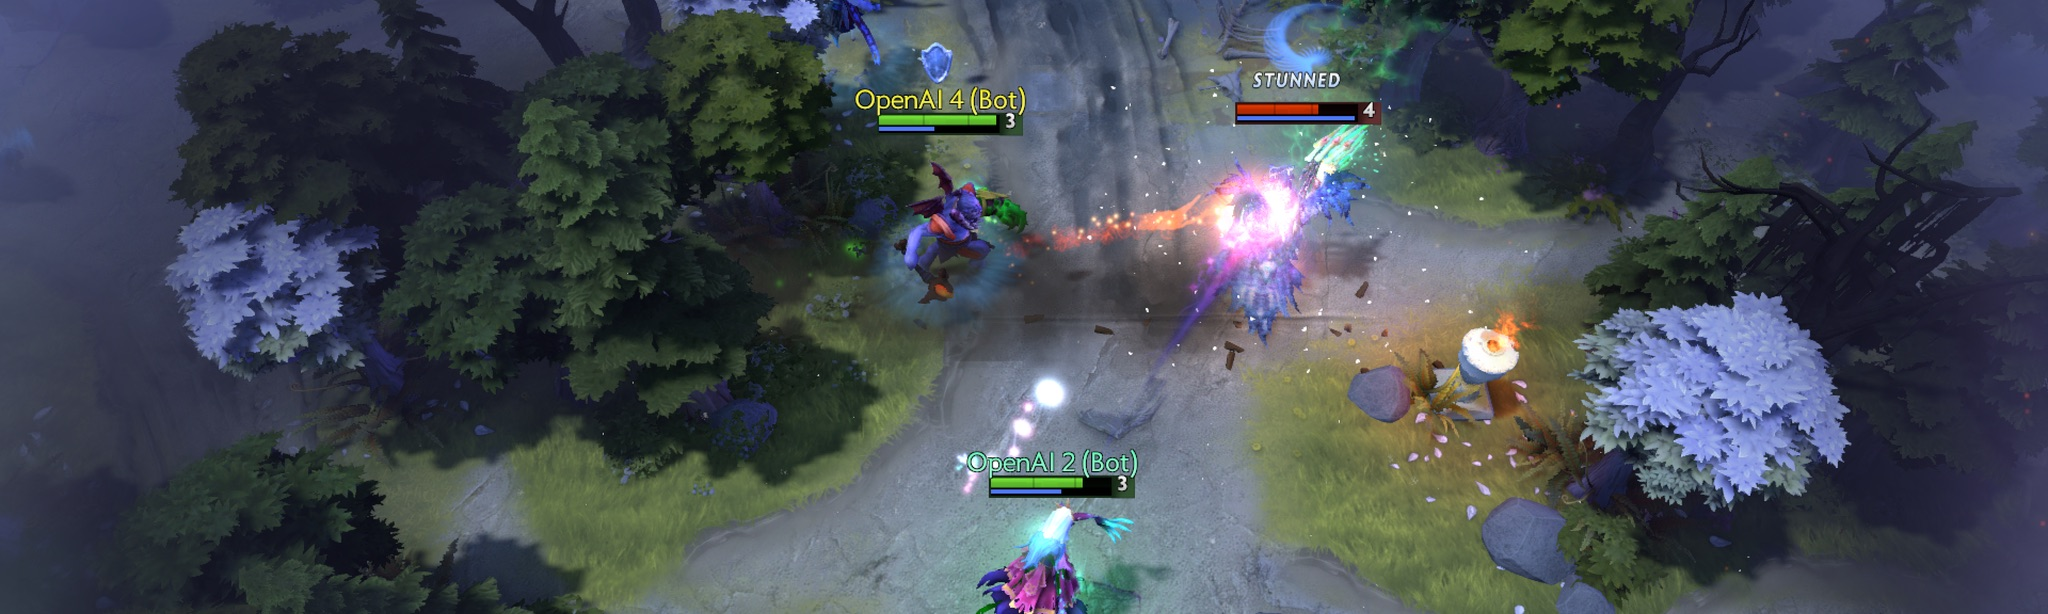
\includegraphics[width=\textwidth]{p2-five}

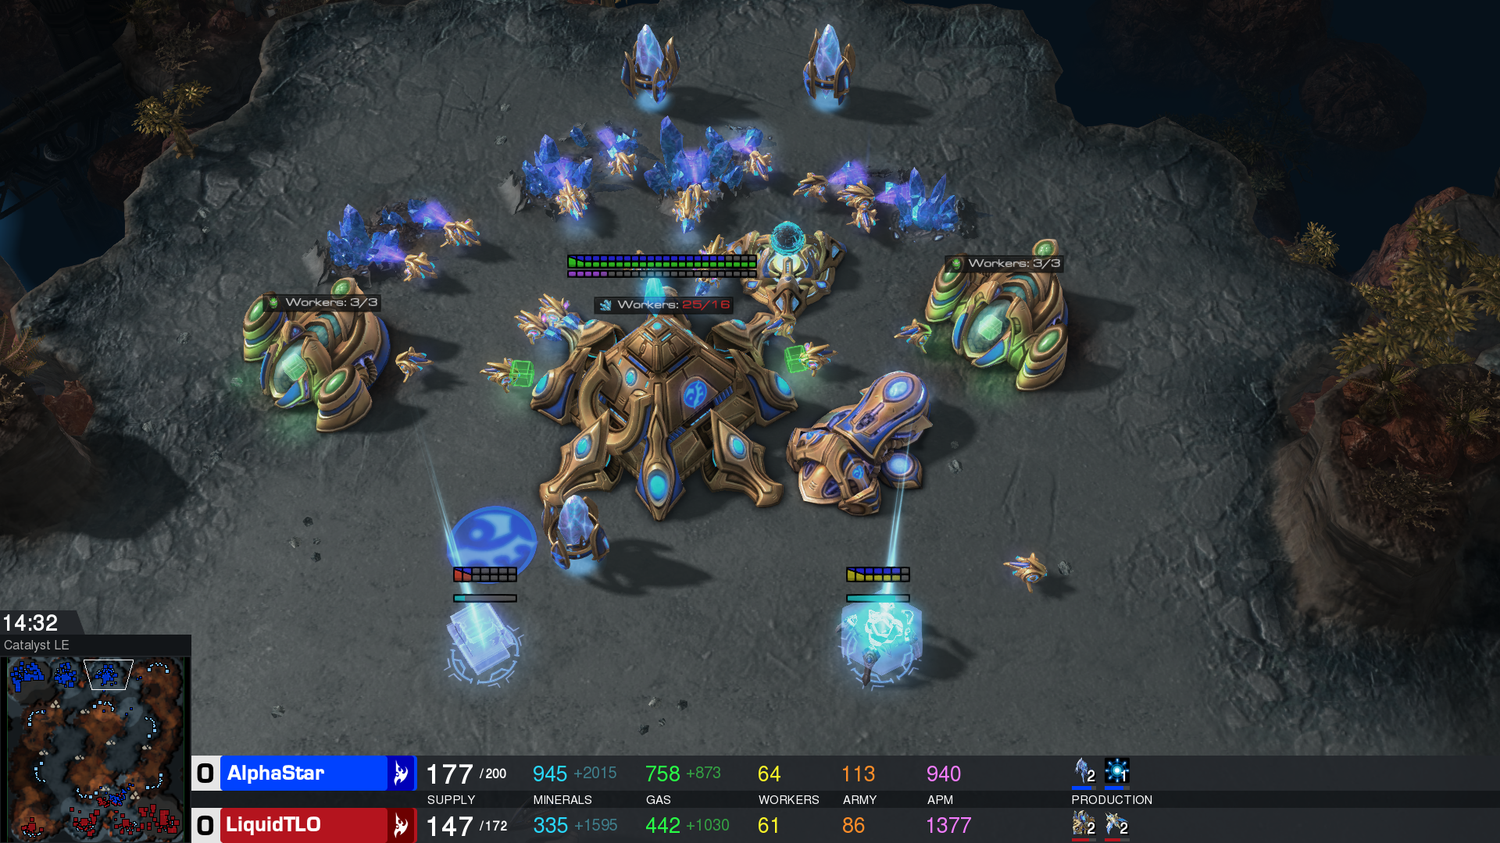
\includegraphics[width=\textwidth]{p2-alphastar}
}
\end{frame}

\begin{frame}{Spotlight on AlphaGo}

\twocolumns{0.6}{0.4}{
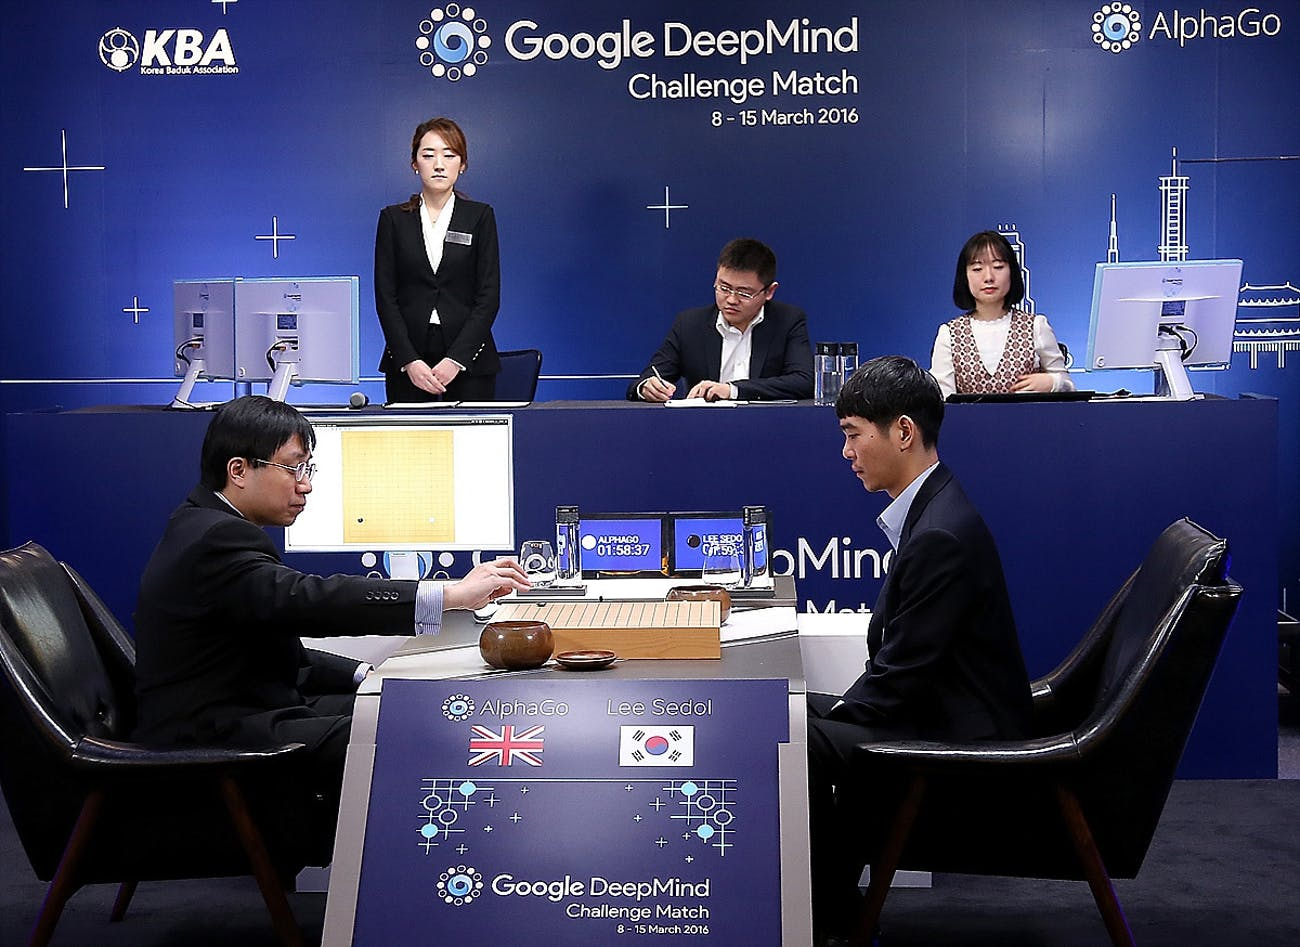
\includegraphics[width=\textwidth]{p2-alphago}
}{
Hard to overstate what an unbelievable accomplishment this was

\vspace{2em}

Previously: Go was considered unassailable stronghold for human experts, AI 10+ years away
}

\end{frame}

\begin{frame}{What RL Can Currently Do: RL in the Real World}

\twocolumns{0.5}{0.5}{
RL is beginning to see profitable real-world applications!
\begin{itemize}
\item Facebook uses RL (DQN) for push notifications (Horizon)
\item DeepMind integrated RL into data center cooling 
\item Several promising early efforts at applying RL for robotics
\end{itemize}
}{


\includegraphics[width=\textwidth]{p2-horizon}


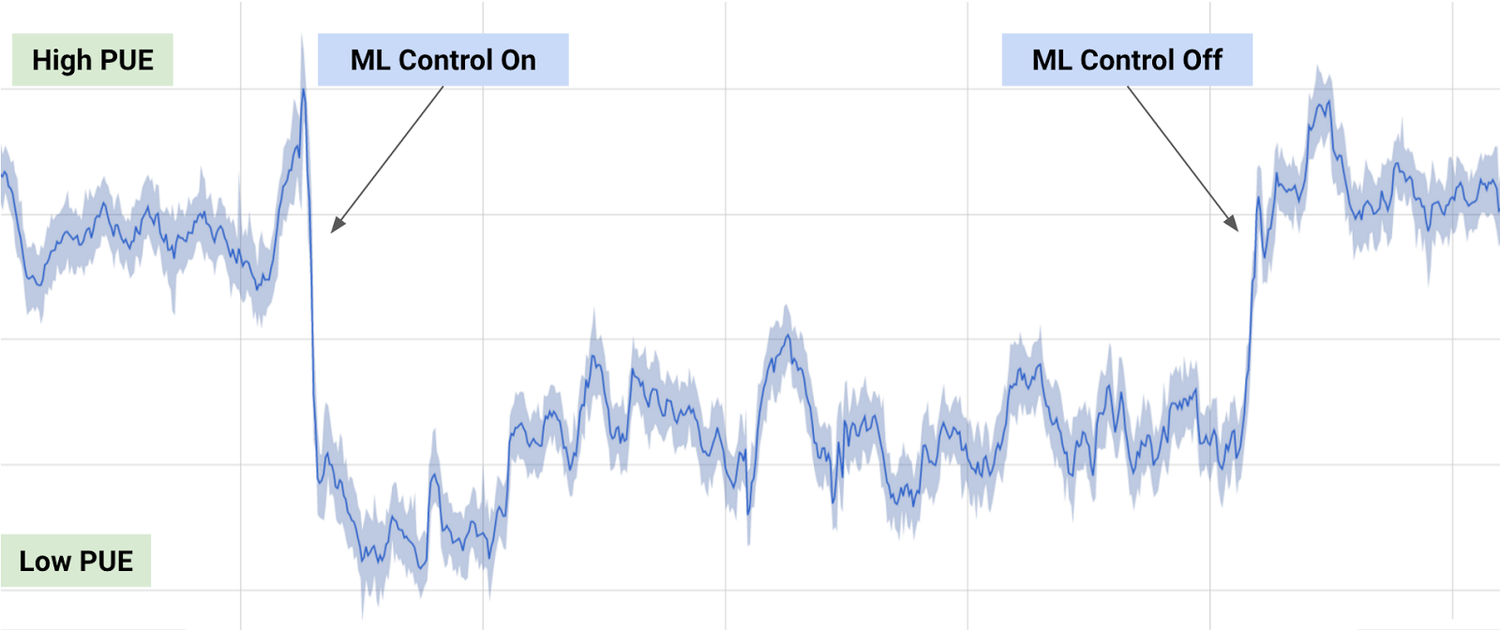
\includegraphics[width=\textwidth]{p2-datacenter}
}

\end{frame}

\section{2.1.1: Spotlight on RL for Real-World Robotics}


\begin{frame}{Tasks that can't easily be simulated}

Zhu et al. trained low-cost robots from scratch in the real world on hard-to-simulate tasks using natural policy gradient. (Note: observation space here is hand state and valve state)

\begin{center}
\movie[width=0.8\textwidth, autostart, loop]{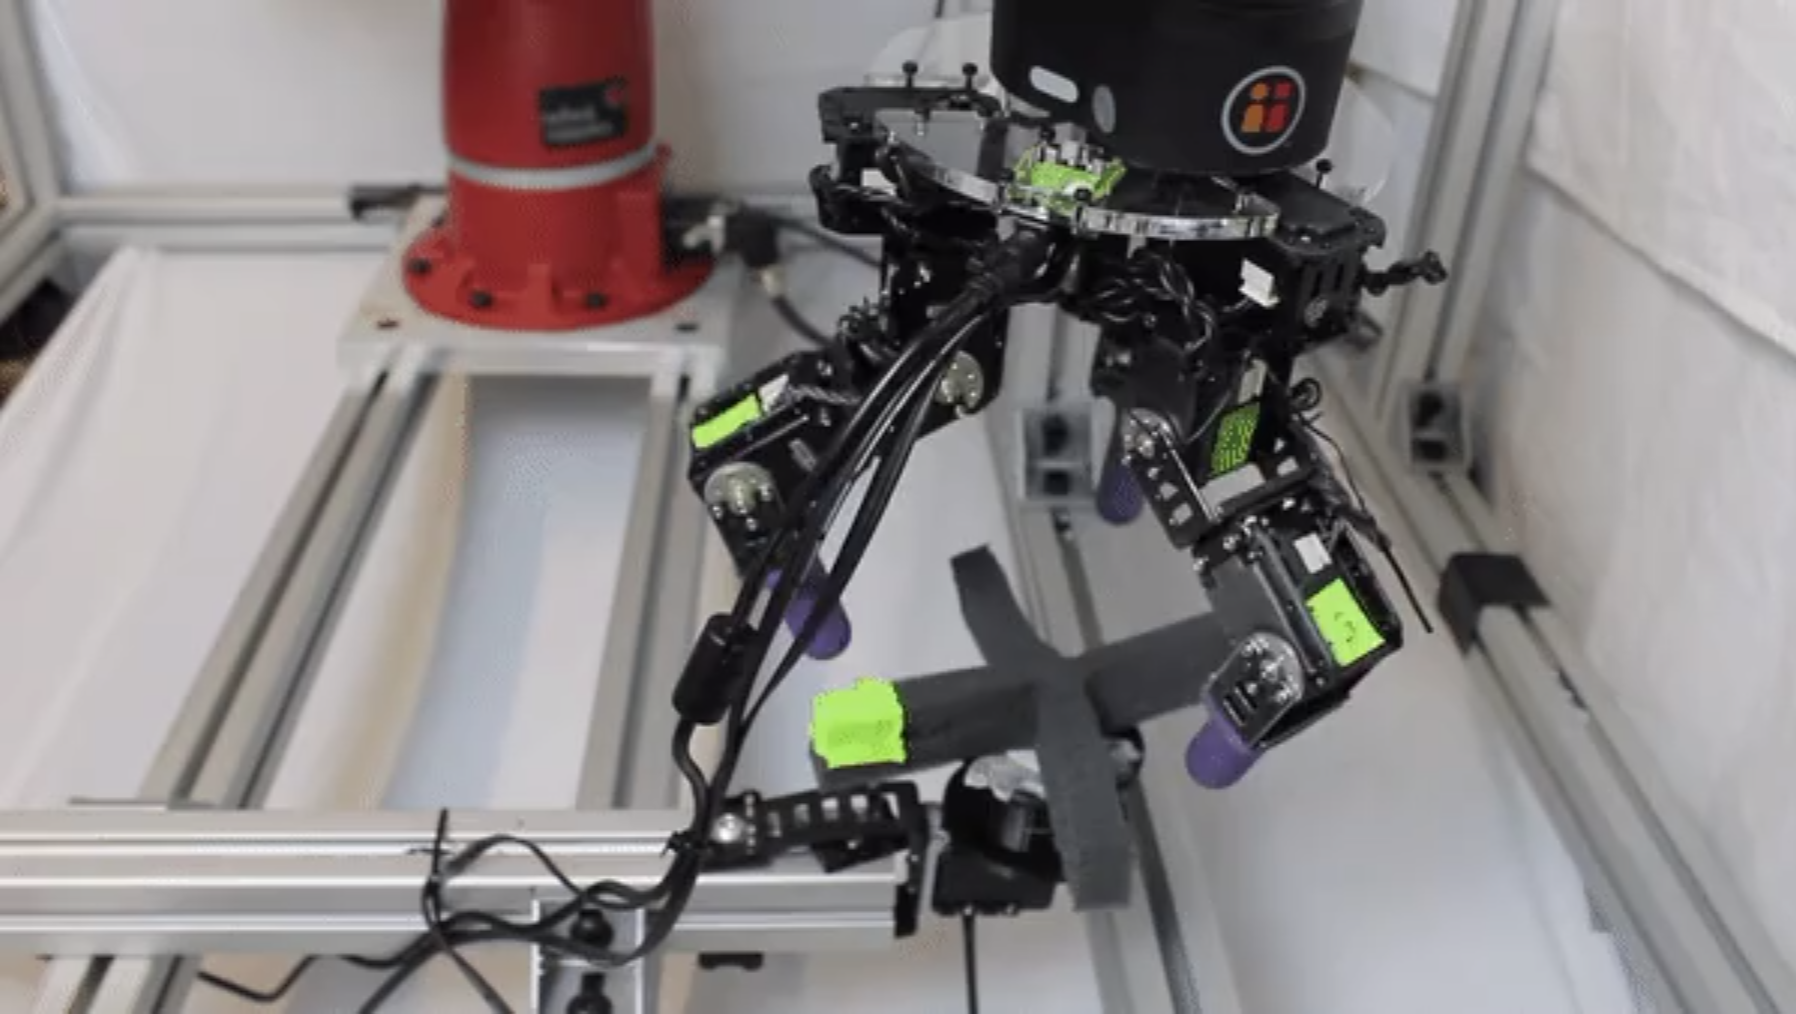
\includegraphics[width=0.8\textwidth]{p2-foamscrew}}{images/p2-foamscrew.mp4}
\end{center}


\footnotemark[1]{Zhu et al, 2018: ``Dexterous Manipulation with Deep Reinforcement Learning: Efficient, General, and Low-Cost"}

\end{frame}

\begin{frame}{Robots that are hard to control conventionally}

Zhang et al. trained a tensegrity robot with deep RL in simulation and demonstrated transfer to the real world
\begin{figure}
\centering
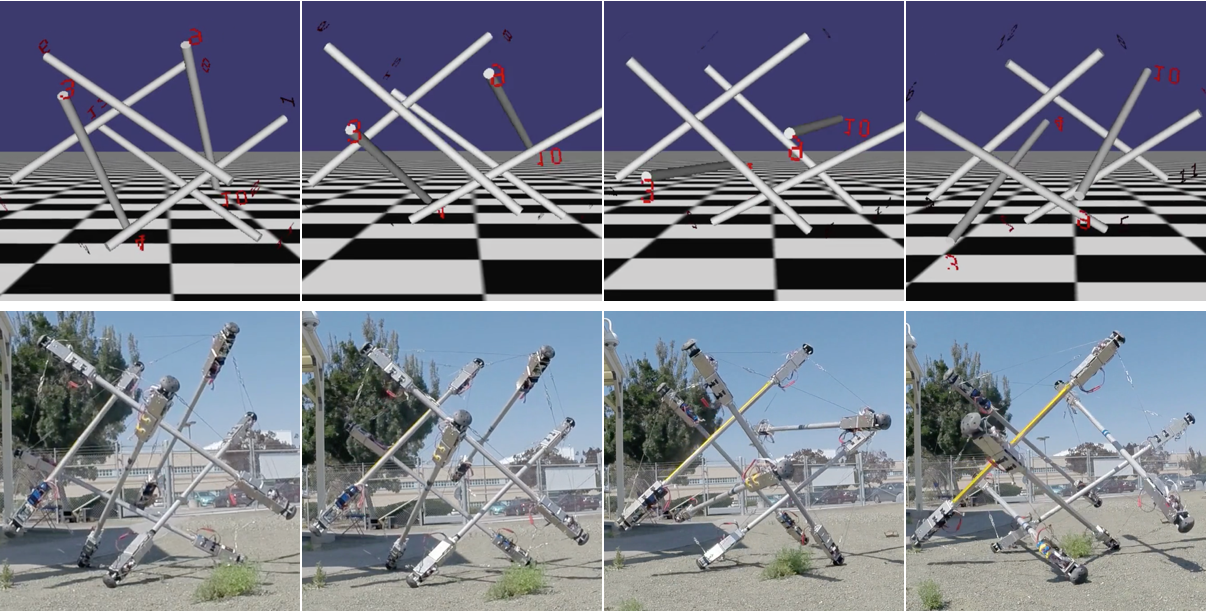
\includegraphics[width=0.8\textwidth]{p2-tensegrity}
\end{figure}


\footnotemark[1]{Zhang et al, 2016: ``Deep Reinforcement Learning for Tensegrity Robot Locomotion"}
\end{frame}

\begin{frame}{Soft Actor-Critic}

Haarnoja et al. trained robots in the real world with Soft Actor-Critic, and demonstrated efficient and robust control on hard domains

\twocolumns{0.5}{0.5}{
\begin{center}
\movie[width=0.9\textwidth, autostart, loop]{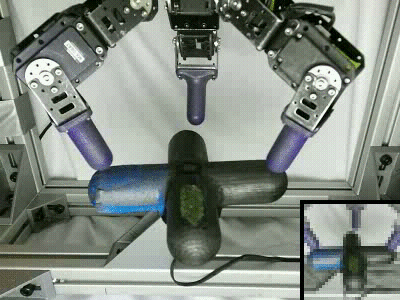
\includegraphics[width=0.9\textwidth]{p2-sac-valve}}{images/p2-sac-valve.mp4}
\end{center}
Manipulation from visual input, agent sees lower-right (took 20 hours to learn)
}{
\begin{center}
\movie[width=\textwidth, autostart, loop]{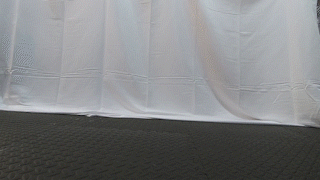
\includegraphics[width=\textwidth]{p2-sac-minitaur}}{images/p2-sac-minitaur.mp4}
\end{center}
Robust control of a legged robot (took 2 hours to learn)
}

\vspace{1em}

\footnotemark[1]{Haarnoja et al, 2018: ``Soft Actor-Critic Algorithms and Applications"}

\end{frame}

\begin{frame}{Anymal}

Hwangbo et al. used real data to learn a better simulator, and then used lots of simulator data to train complex locomotion and recovery policies with TRPO for the Anymal robot:

\begin{center}
\movie[width=0.8\textwidth, autostart, loop]{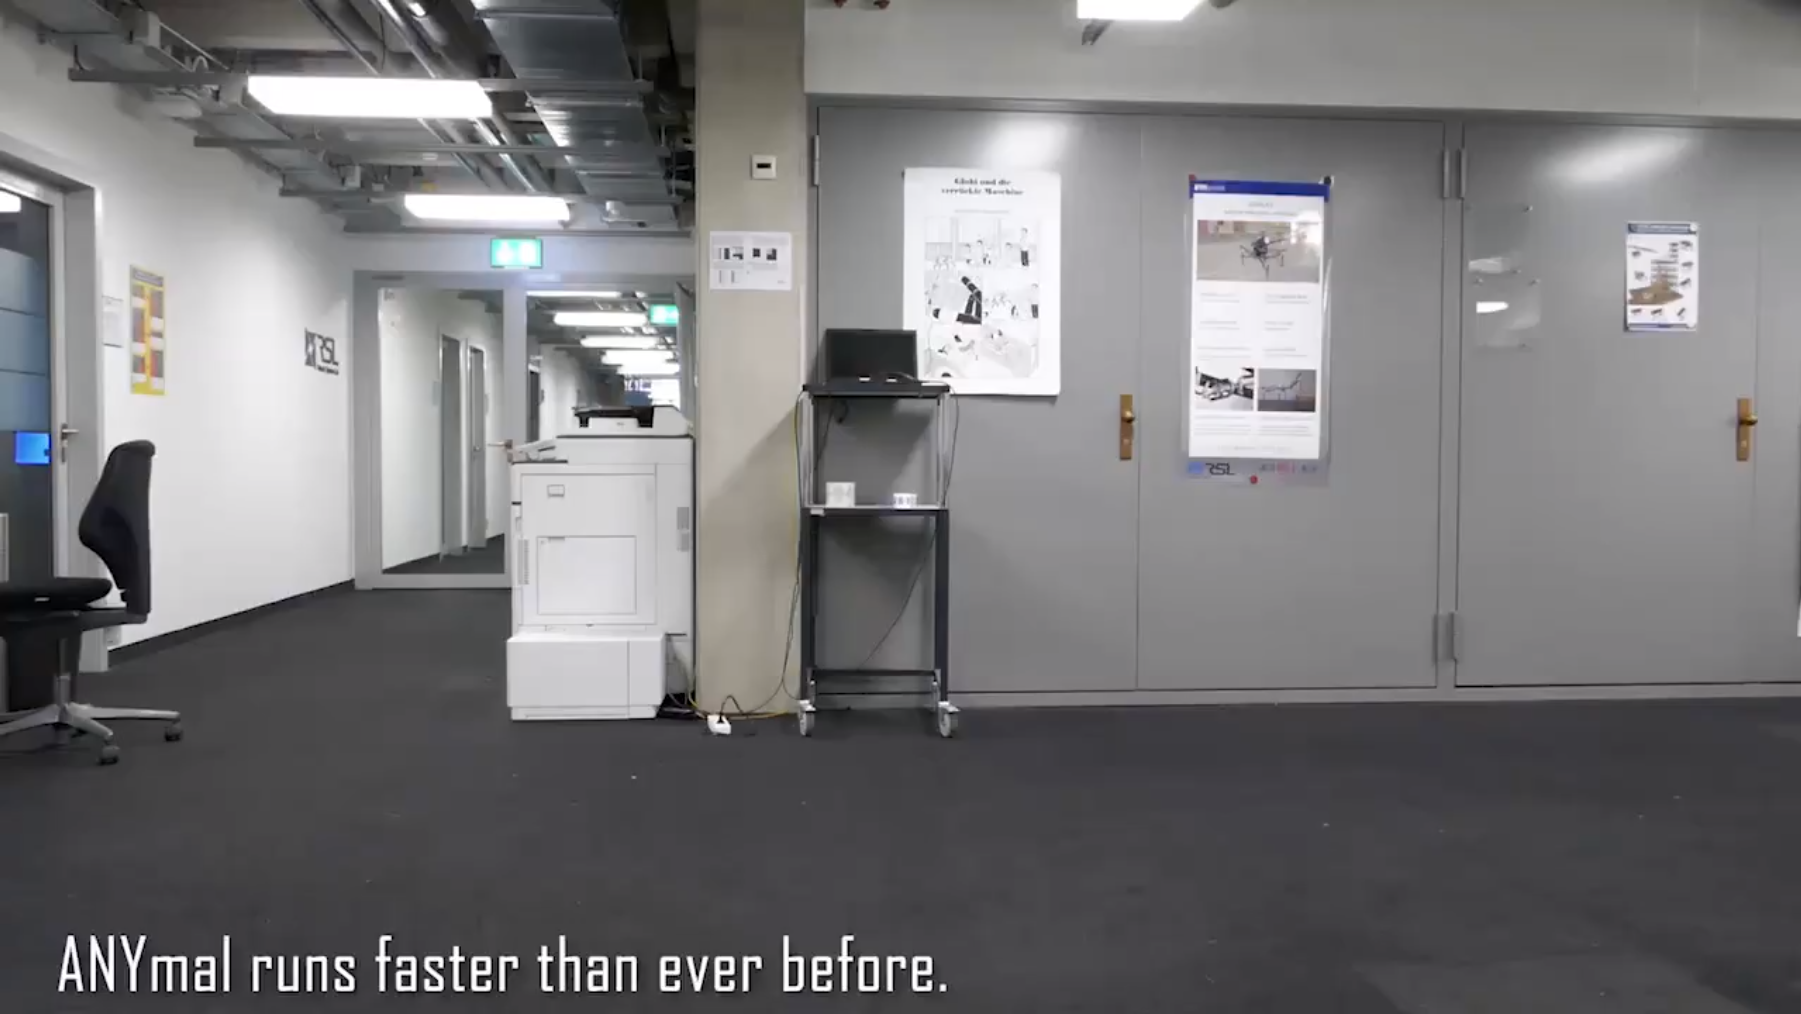
\includegraphics[width=0.8\textwidth]{p2-anymal}}{images/p2-anymal.mp4}
\end{center}

\footnotemark[1]{Hwangbo et al, 2018: ``Learning agile and dynamic motor skills for legged robots"}
\end{frame}

\begin{frame}{Learning Dexterity}

OpenAI et al. trained policies with PPO to dextrously manipulate a complex hand robot, using sim2real by domain randomization:

\begin{center}
\movie[width=0.8\textwidth, autostart, loop]{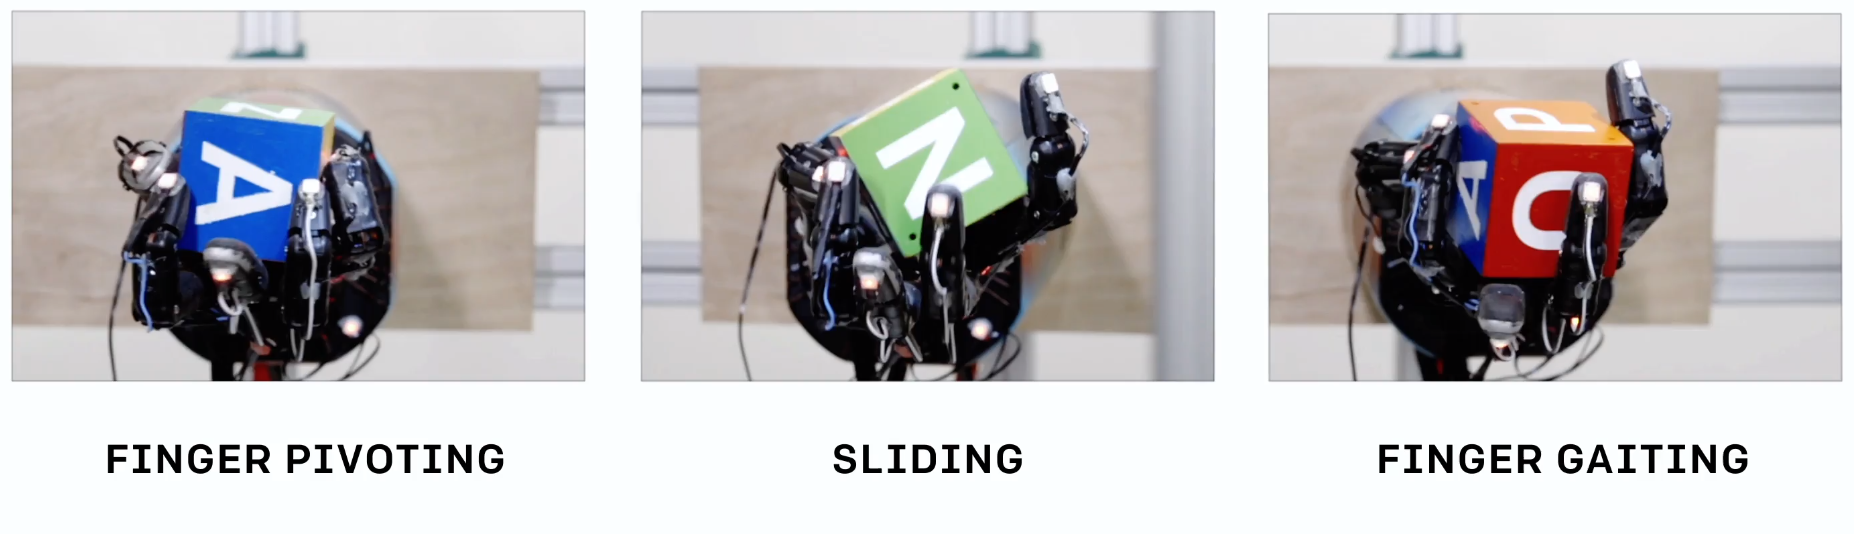
\includegraphics[width=0.8\textwidth]{p2-dexterity}}{images/p2-dexterity.mov}
\end{center}

\footnotemark[1]{OpenAI et al, 2018: ``Learning Dexterous In-Hand Manipulation"}

\end{frame}

\section{2.2: What are the challenges in modern RL?}

\begin{frame}{Some grand challenges for RL}

Let's talk about where RL fails, what we need that we aren't getting, and what research is happening.

\begin{itemize}
\item \textbf{Sample efficiency}: Modern deep RL algorithms are very inefficient with data, requiring in some cases 100x or more experience than a human to achieve good performance. How can we make them faster?
\pause
\item \textbf{Exploration}: Modern RL is terrible at environments where rewards are very rare---how can we get agents to try out new things?
\pause
\item \textbf{Generalization}: Policies trained for one task are brittle and cannot be used outside of training environment: how can we make them generalize?
\pause
\item \textbf{Safety}: How can we make sure that agents trained by deep RL behave in ways consistent with human preferences?
\end{itemize}

\end{frame}

\section{2.2.1: Research on Improving Sample Efficiency}

\begin{frame}{Combining Model-Free Improvements}
\twocolumns{0.5}{0.5}{
\textbf{Rainbow DQN}: combines...
\begin{itemize}
\item Dueling architecture
\item Double Q-Learning
\item Prioritized experience replay
\item N-step Q-Learning
\item Distributional Q-Learning
\item Parameter-space noise
\end{itemize}
}{
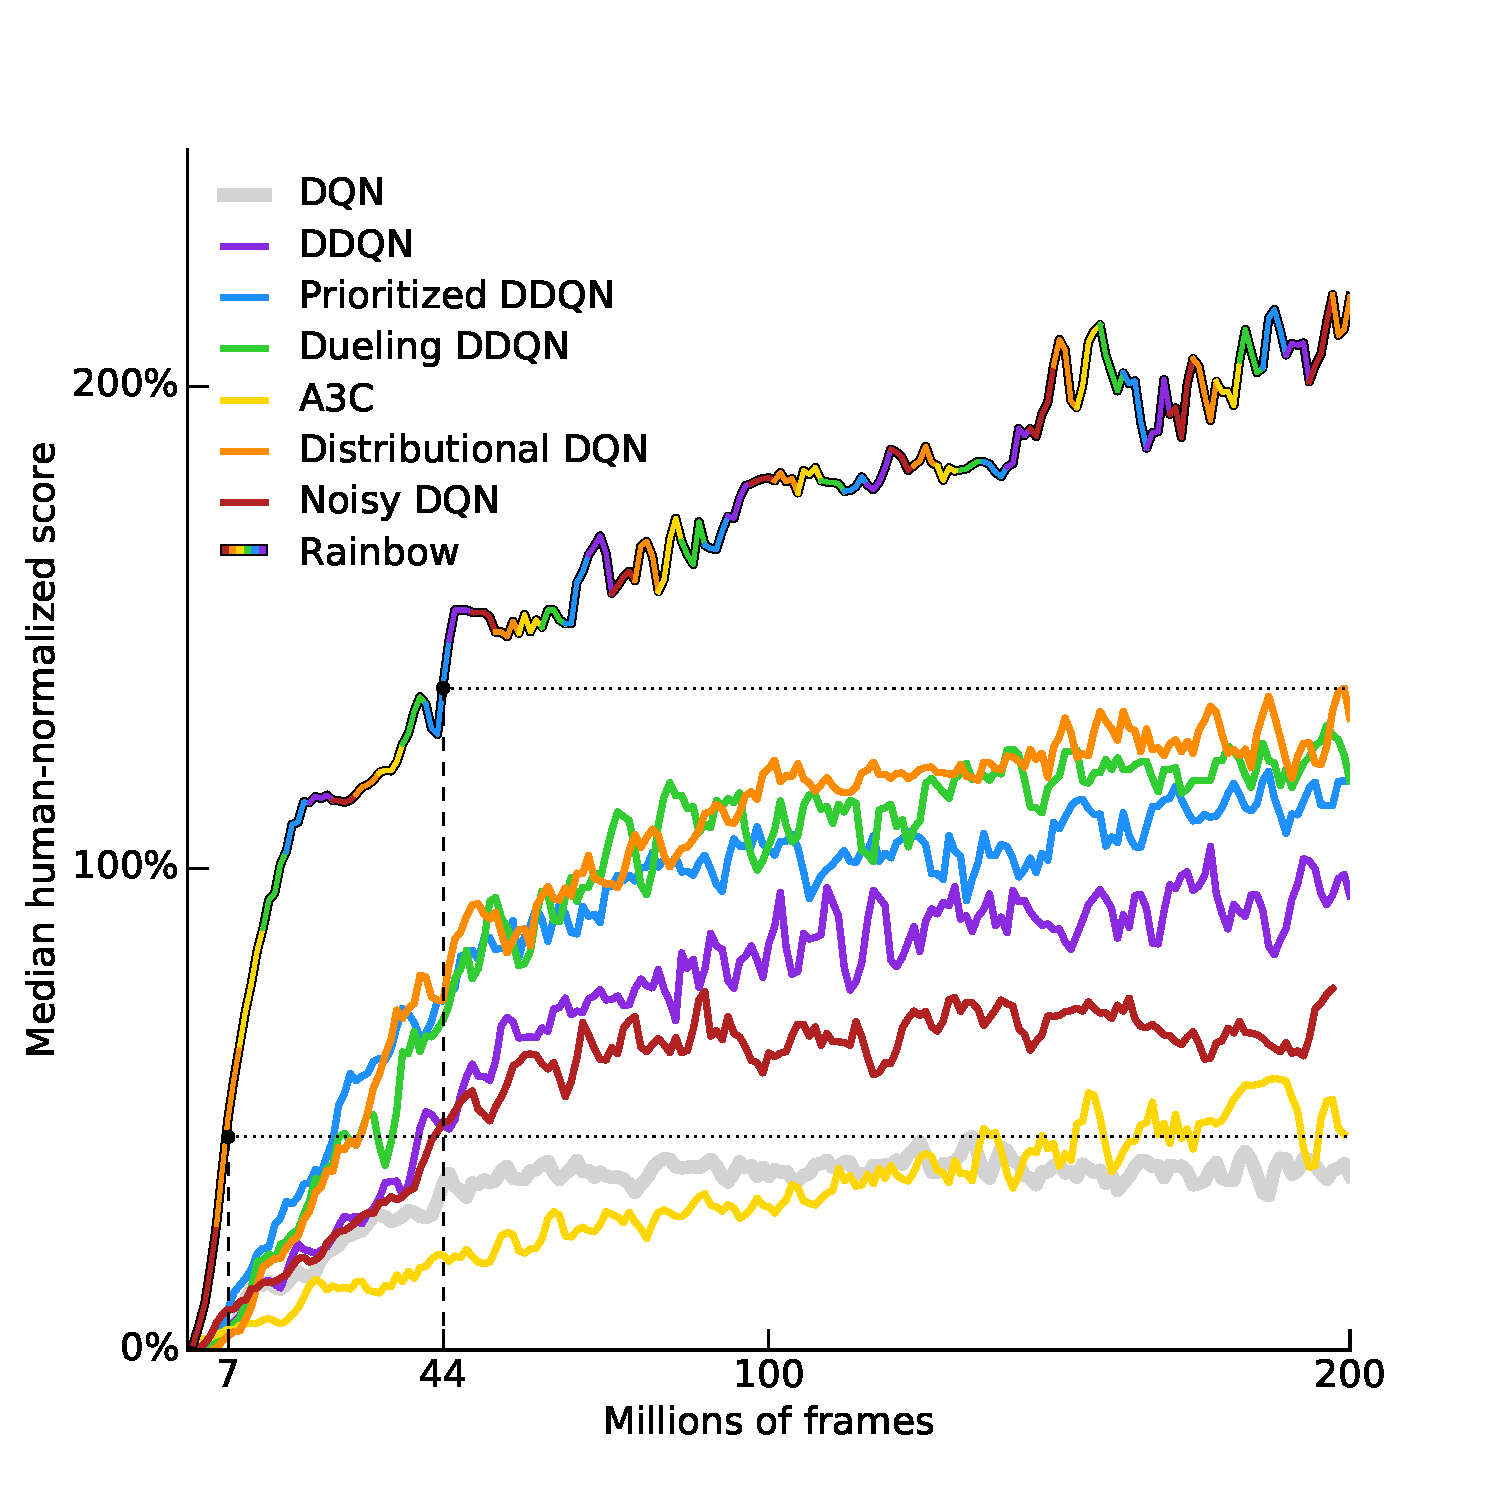
\includegraphics[width=\textwidth]{p2-rainbow}
}
\footnotemark[1]{Hessel et al, 2017: ``Rainbow: Combining Improvements in Deep Reinforcement Learning"}

\end{frame}

\begin{frame}{Accelerating Feature Learning with Unsupervised Learning}

\textbf{UNREAL} uses various unsupervised auxilliary tasks to speed up learning:

\twocolumns{0.5}{0.5}{
\begin{center}
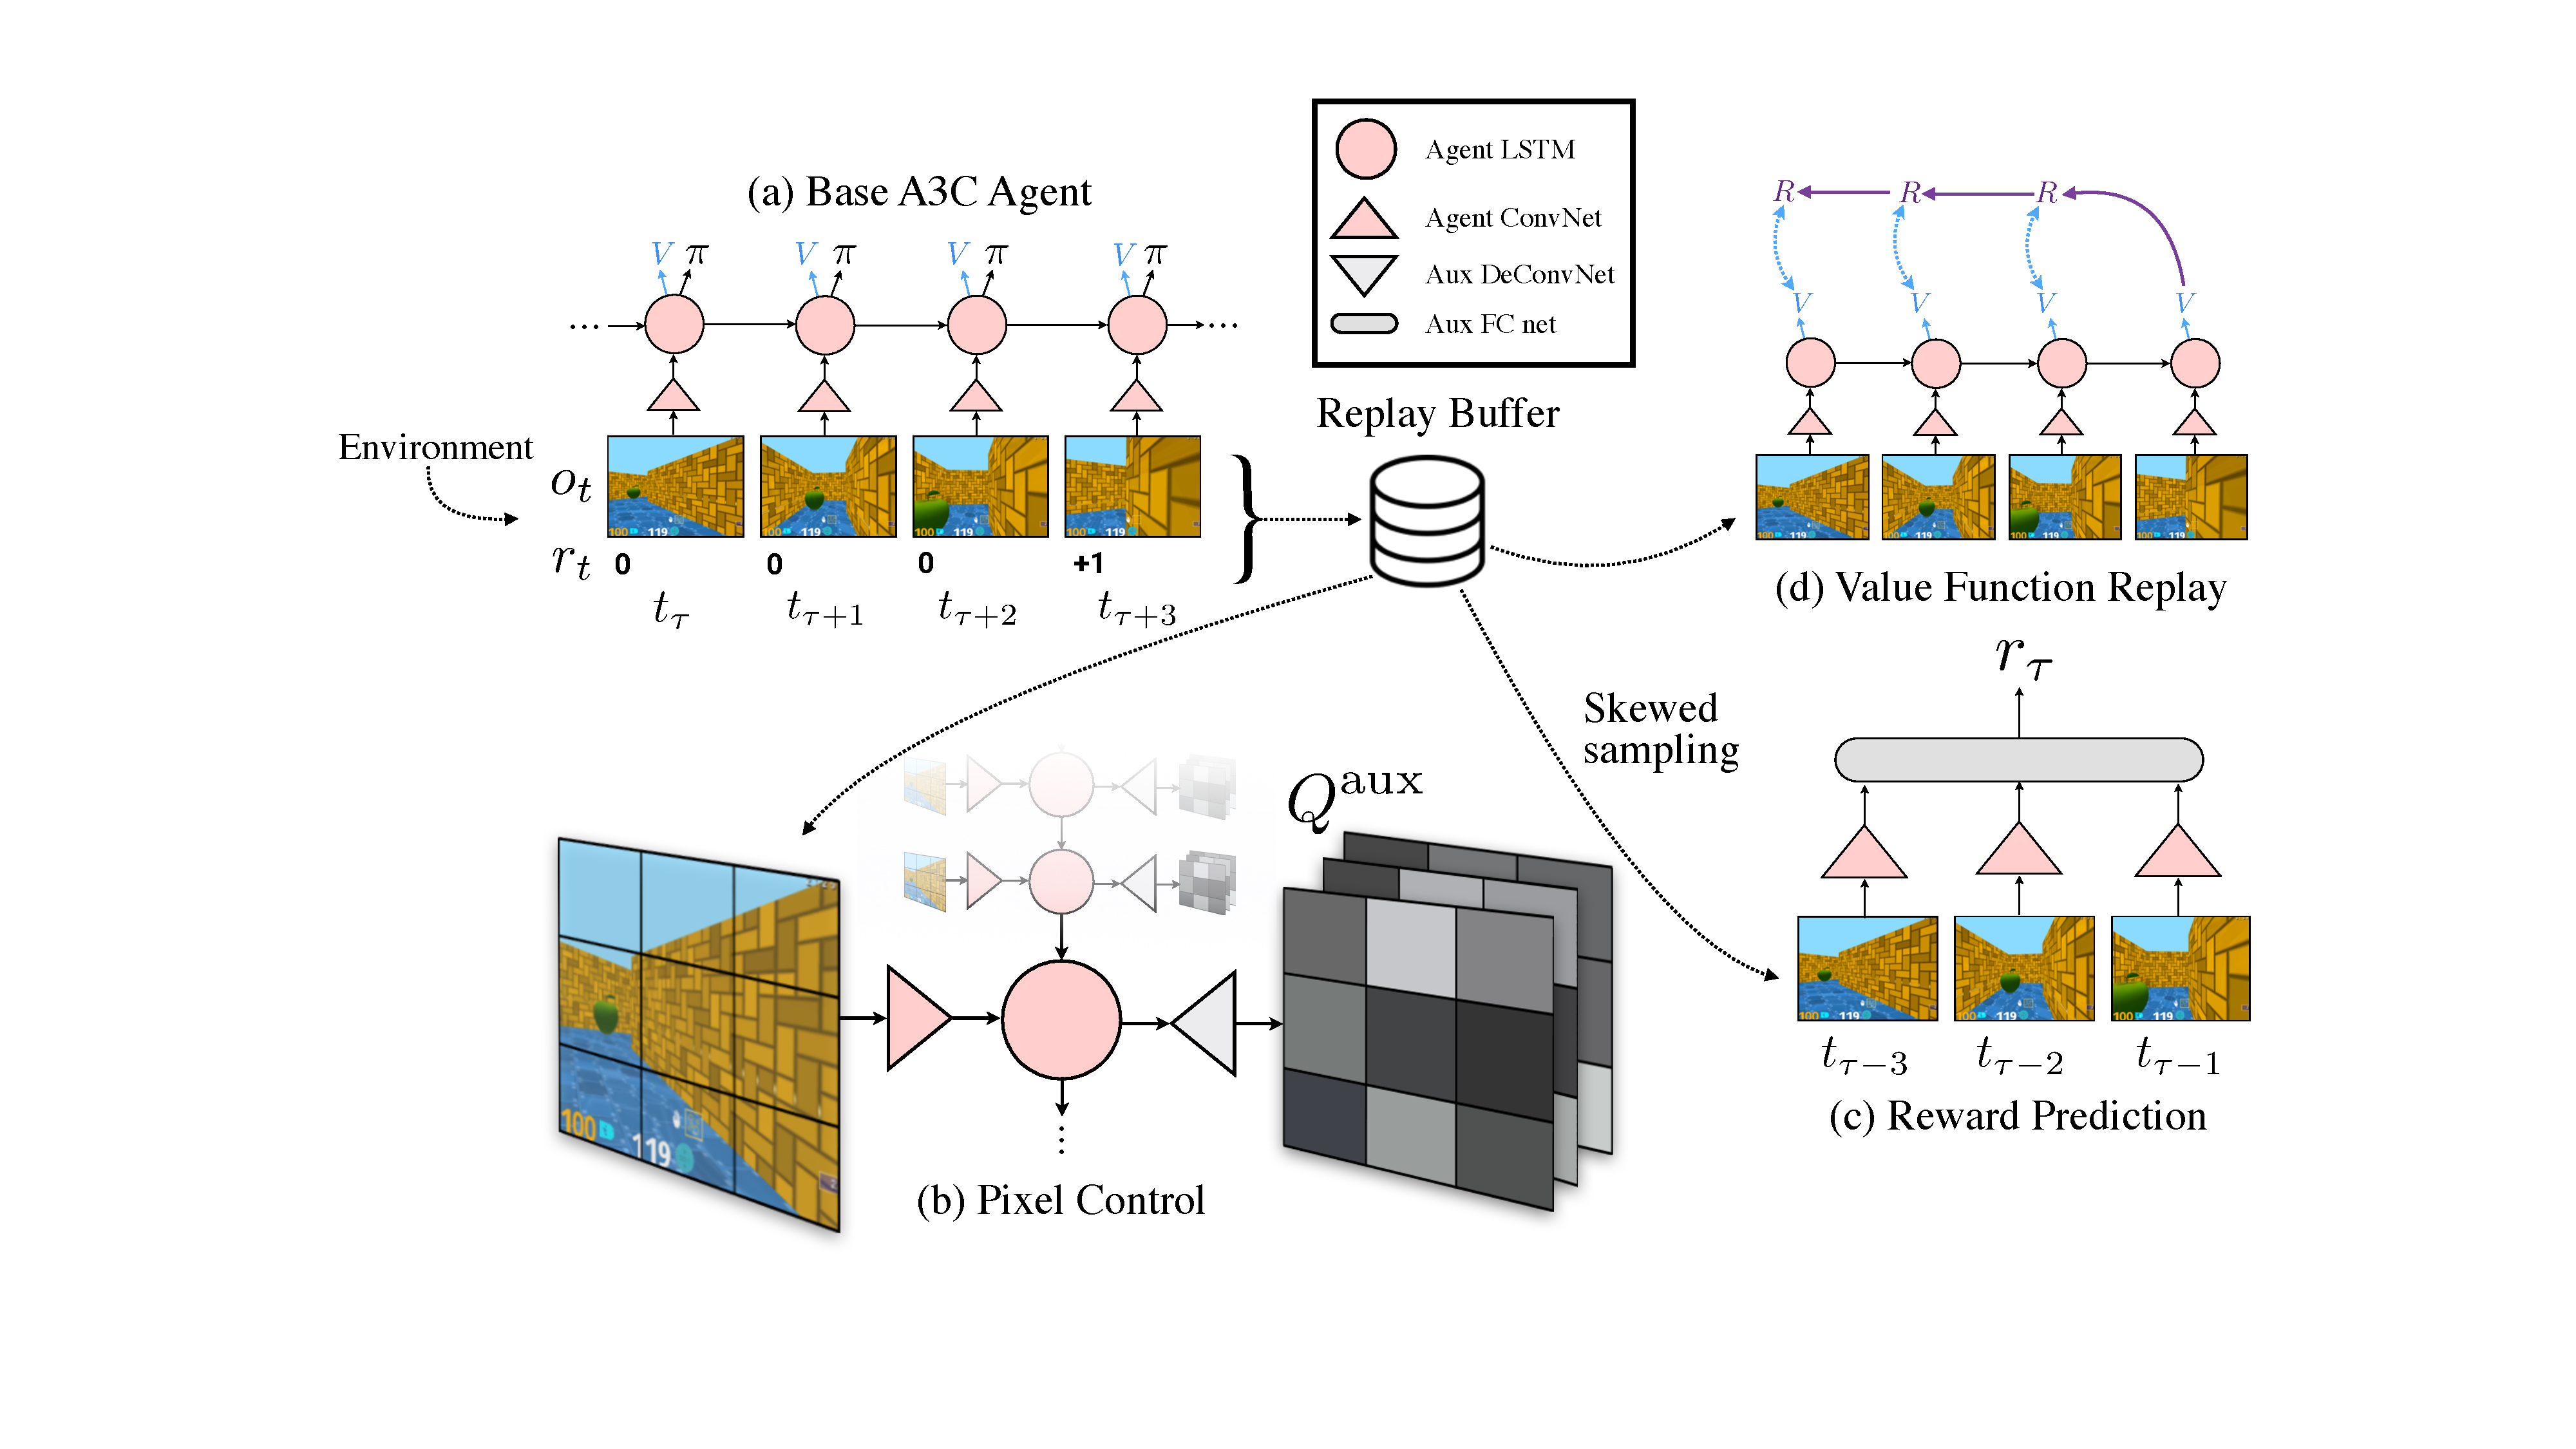
\includegraphics[width=0.9\textwidth]{p2-unreal2}
\end{center}
}{
\begin{center}
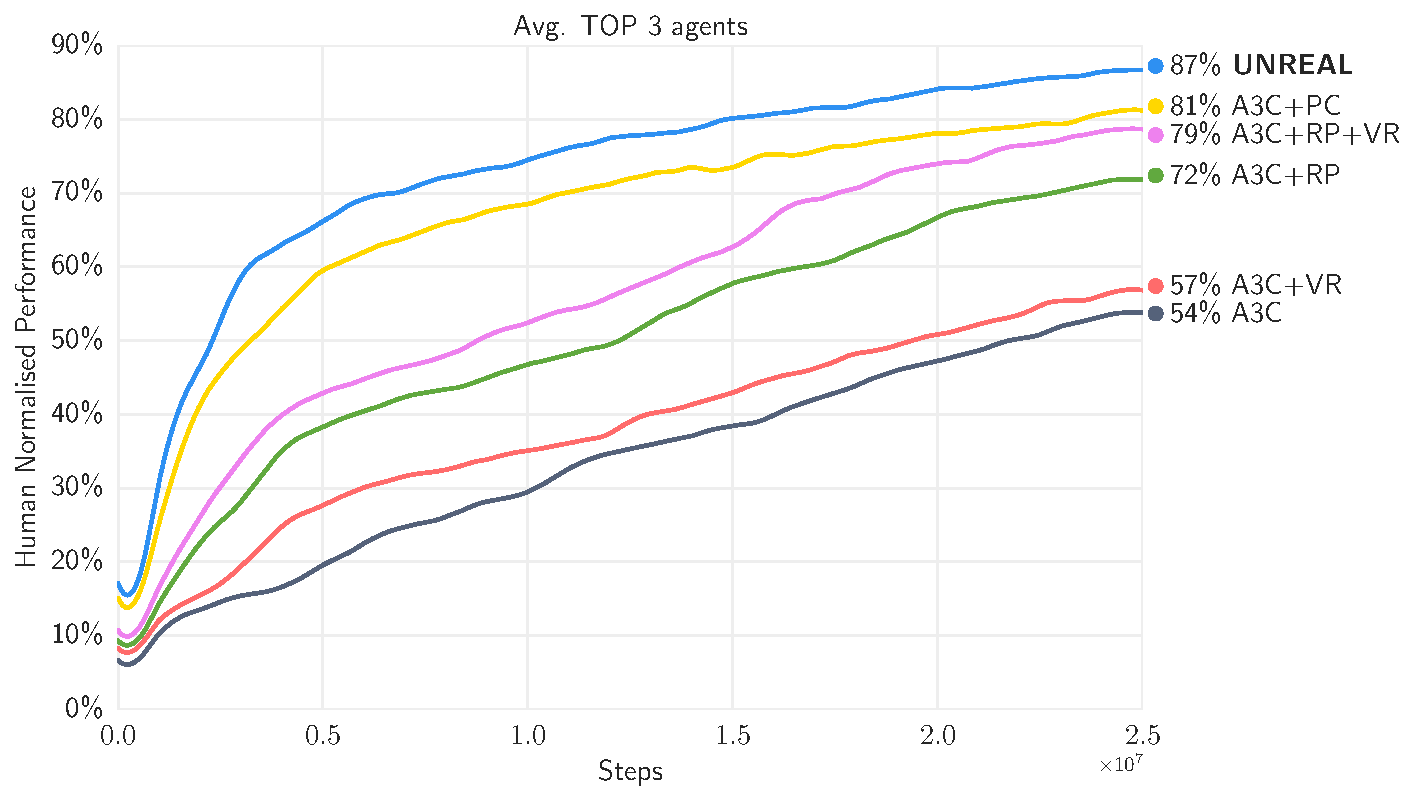
\includegraphics[width=0.9\textwidth]{p2-unreal-labyrinth}
\end{center}
}
\vspace{1em}

\footnotemark[1]{Jaderberg et al, 2016: ``Reinforcement Learning with Unsupervised Auxiliary Tasks"}


%
%\begin{center}
%\movie[width=0.8\textwidth, autostart, loop]{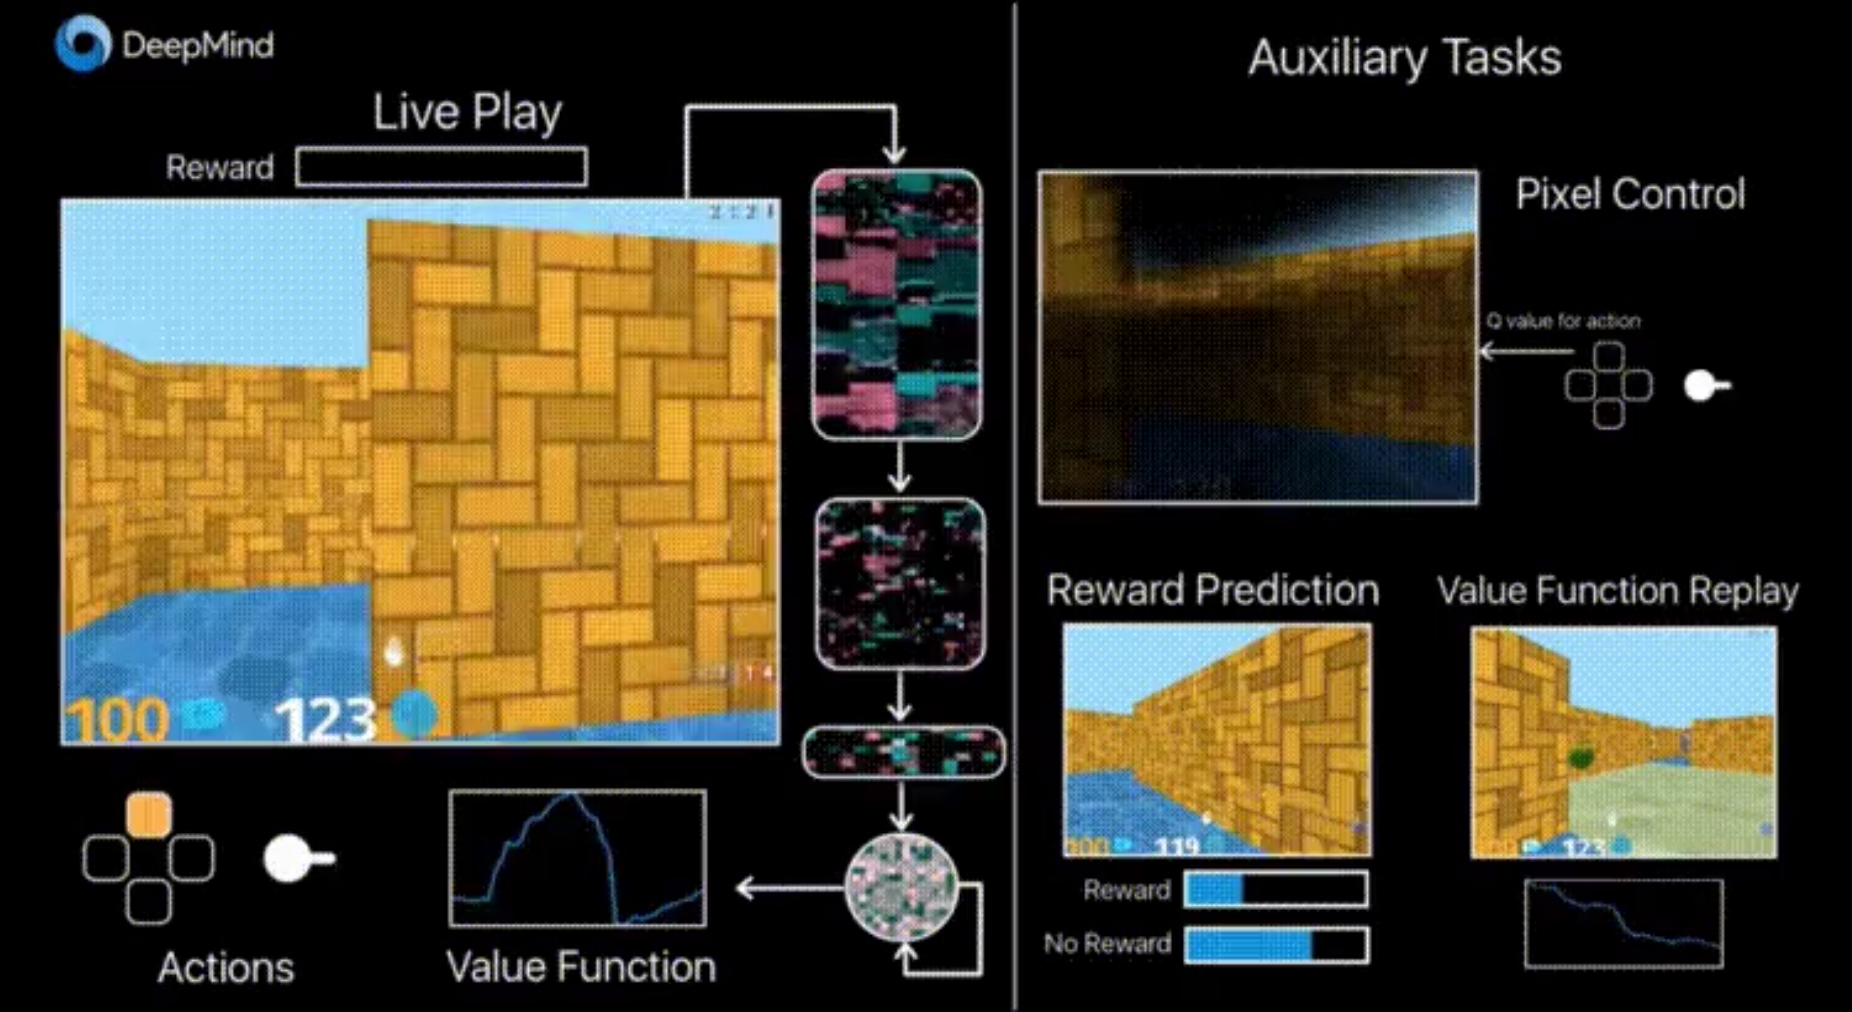
\includegraphics[width=0.8\textwidth]{p2-unreal}}{images/p2-unreal.mp4}
%\end{center}

\end{frame}

\begin{frame}{Combining with Memory Mechanisms}

\textbf{MERLIN} combines unsupervised learning and attention-based memory to improve over baseline architectures:

\twocolumns{0.5}{0.5}{
\begin{center}
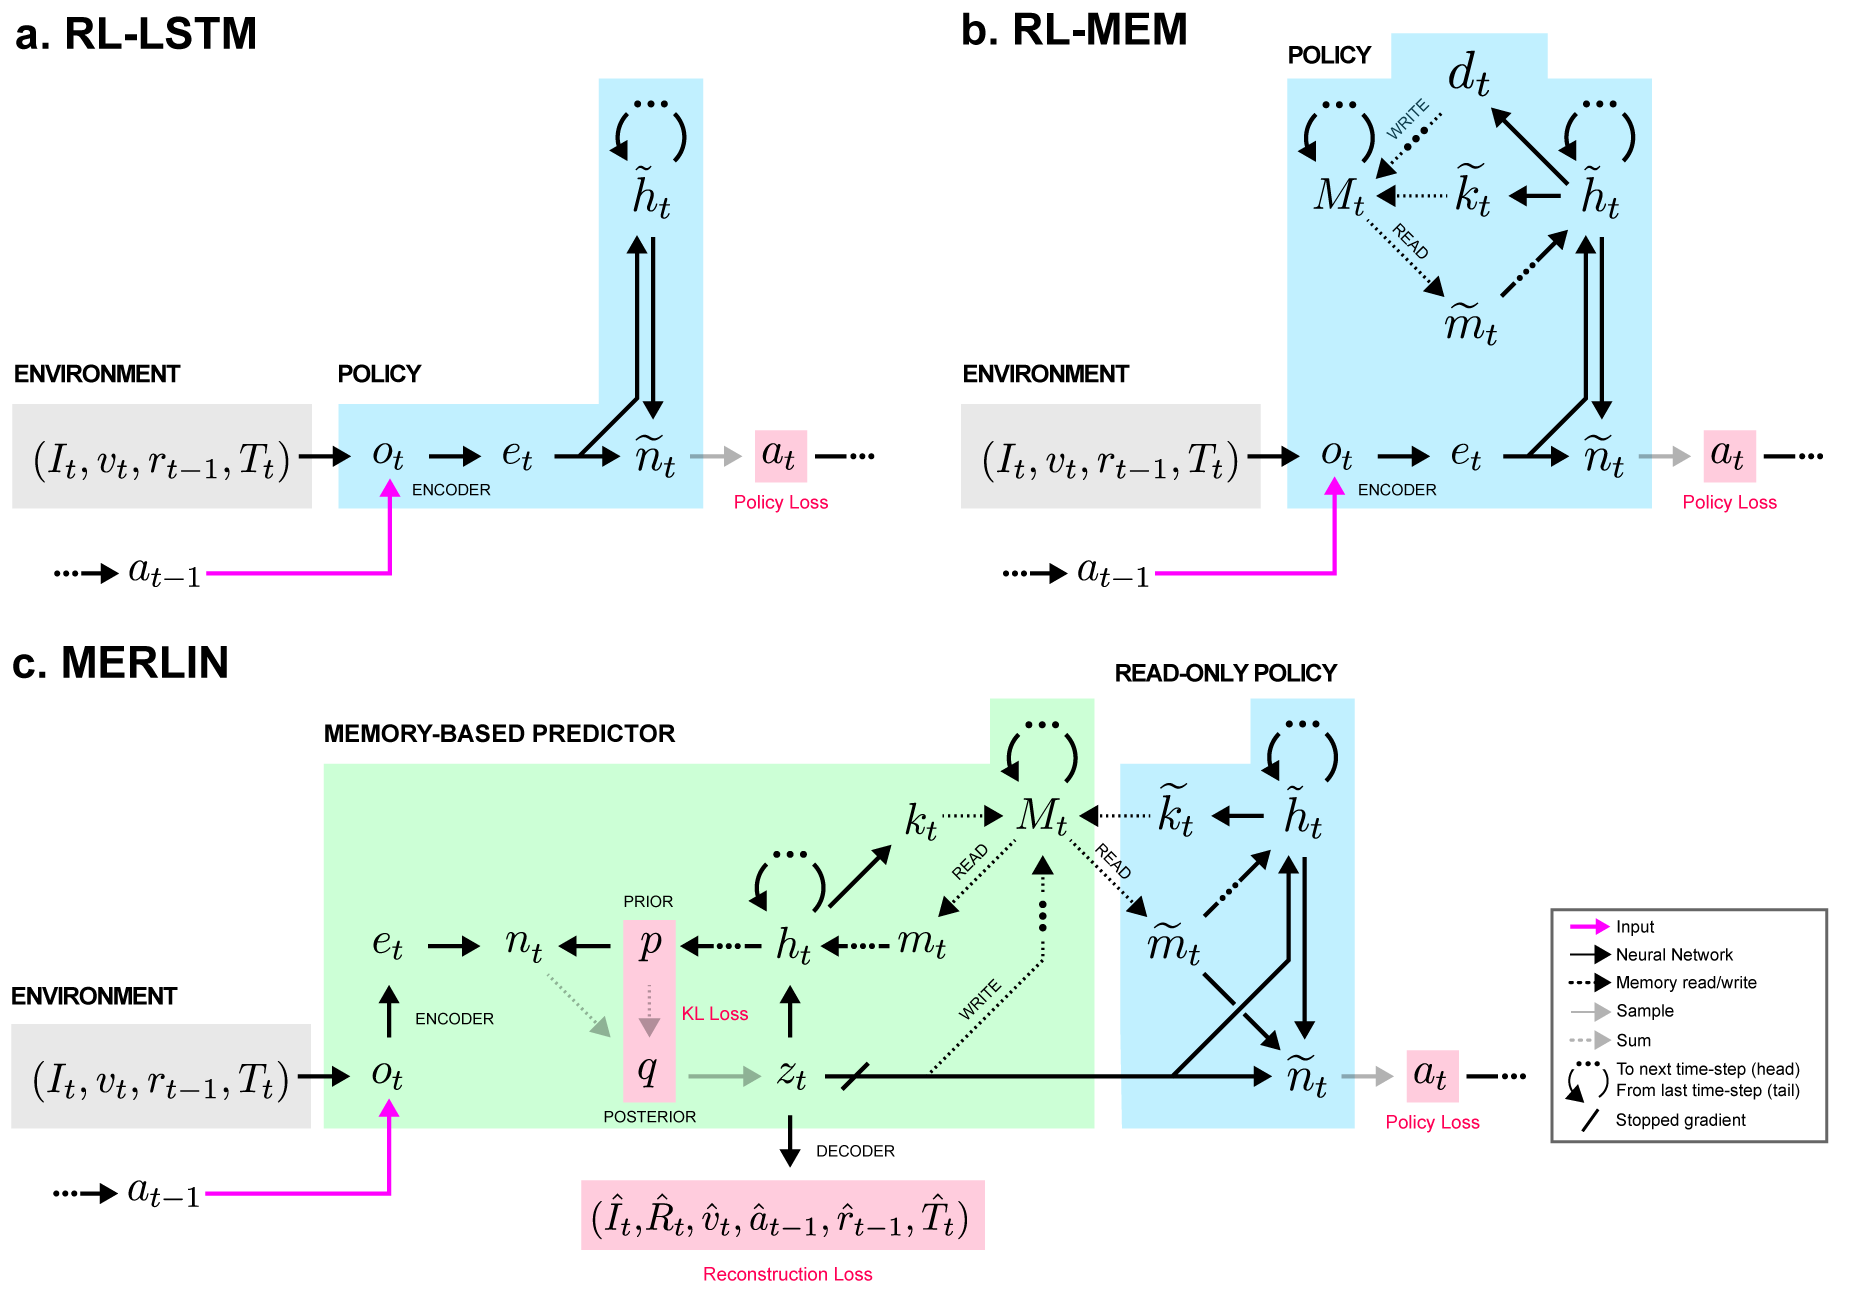
\includegraphics[width=0.9\textwidth]{p2-merlin1}
\end{center}
}{
\begin{center}
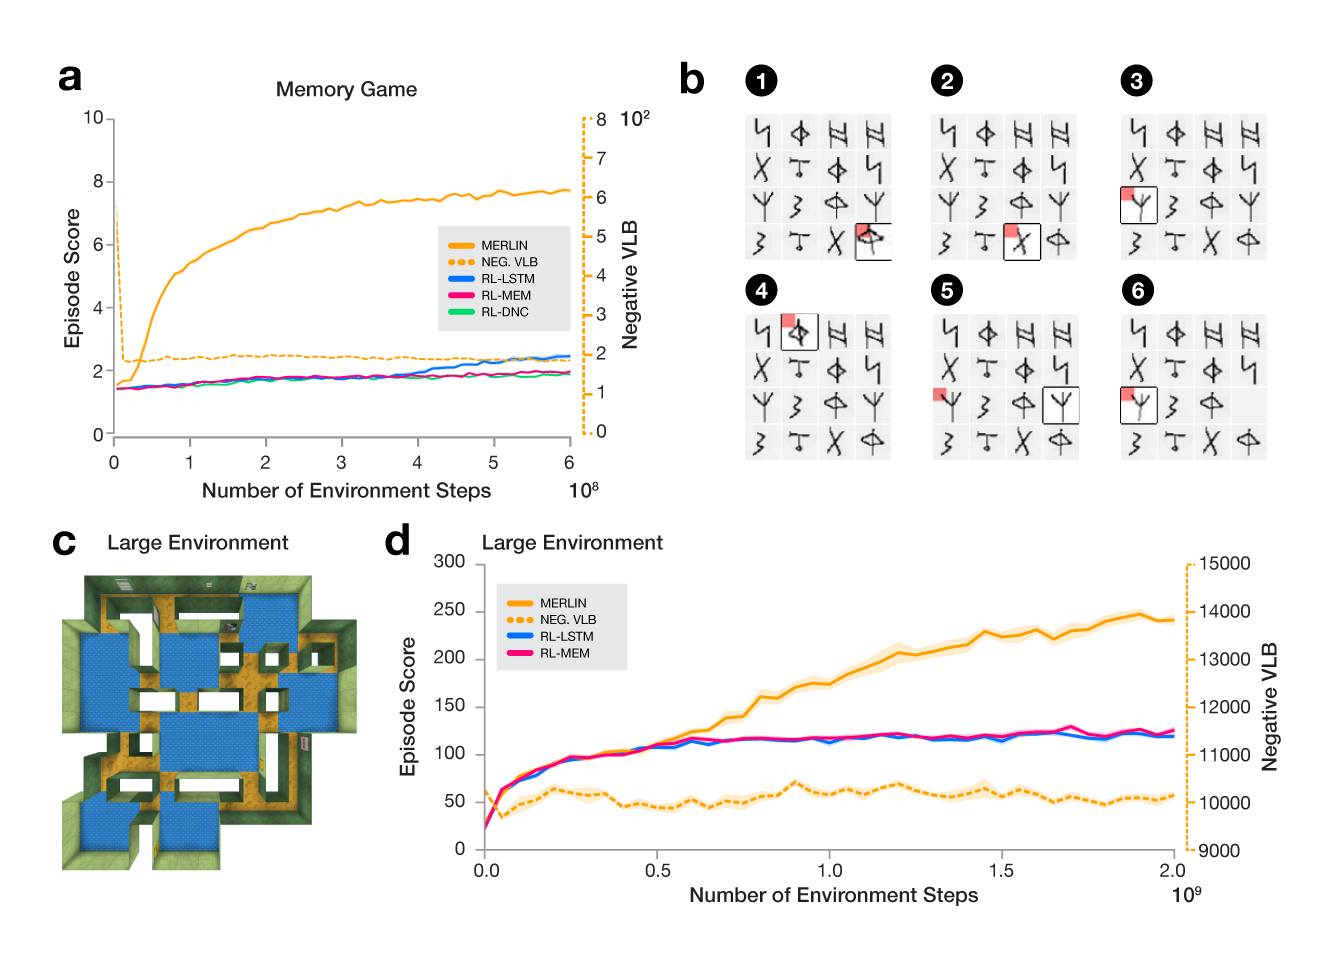
\includegraphics[width=0.9\textwidth]{p2-merlin2}
\end{center}
}

Note: this avenue may not help on arbitrary problems, but seems likely to help on sophisticated partially-observed ones
\vspace{1em}

\footnotemark[1]{Wayne et al, 2018: ``Unsupervised Predictive Memory in a Goal-Directed Agent"}

\end{frame}

\begin{frame}{Model-Based RL}

Techniques like \textbf{World Models}, that allow an agent to learn from simulated experience, are another way to bring down the needed number of real samples:

\begin{center}
\movie[width=0.8\textwidth, autostart, loop]{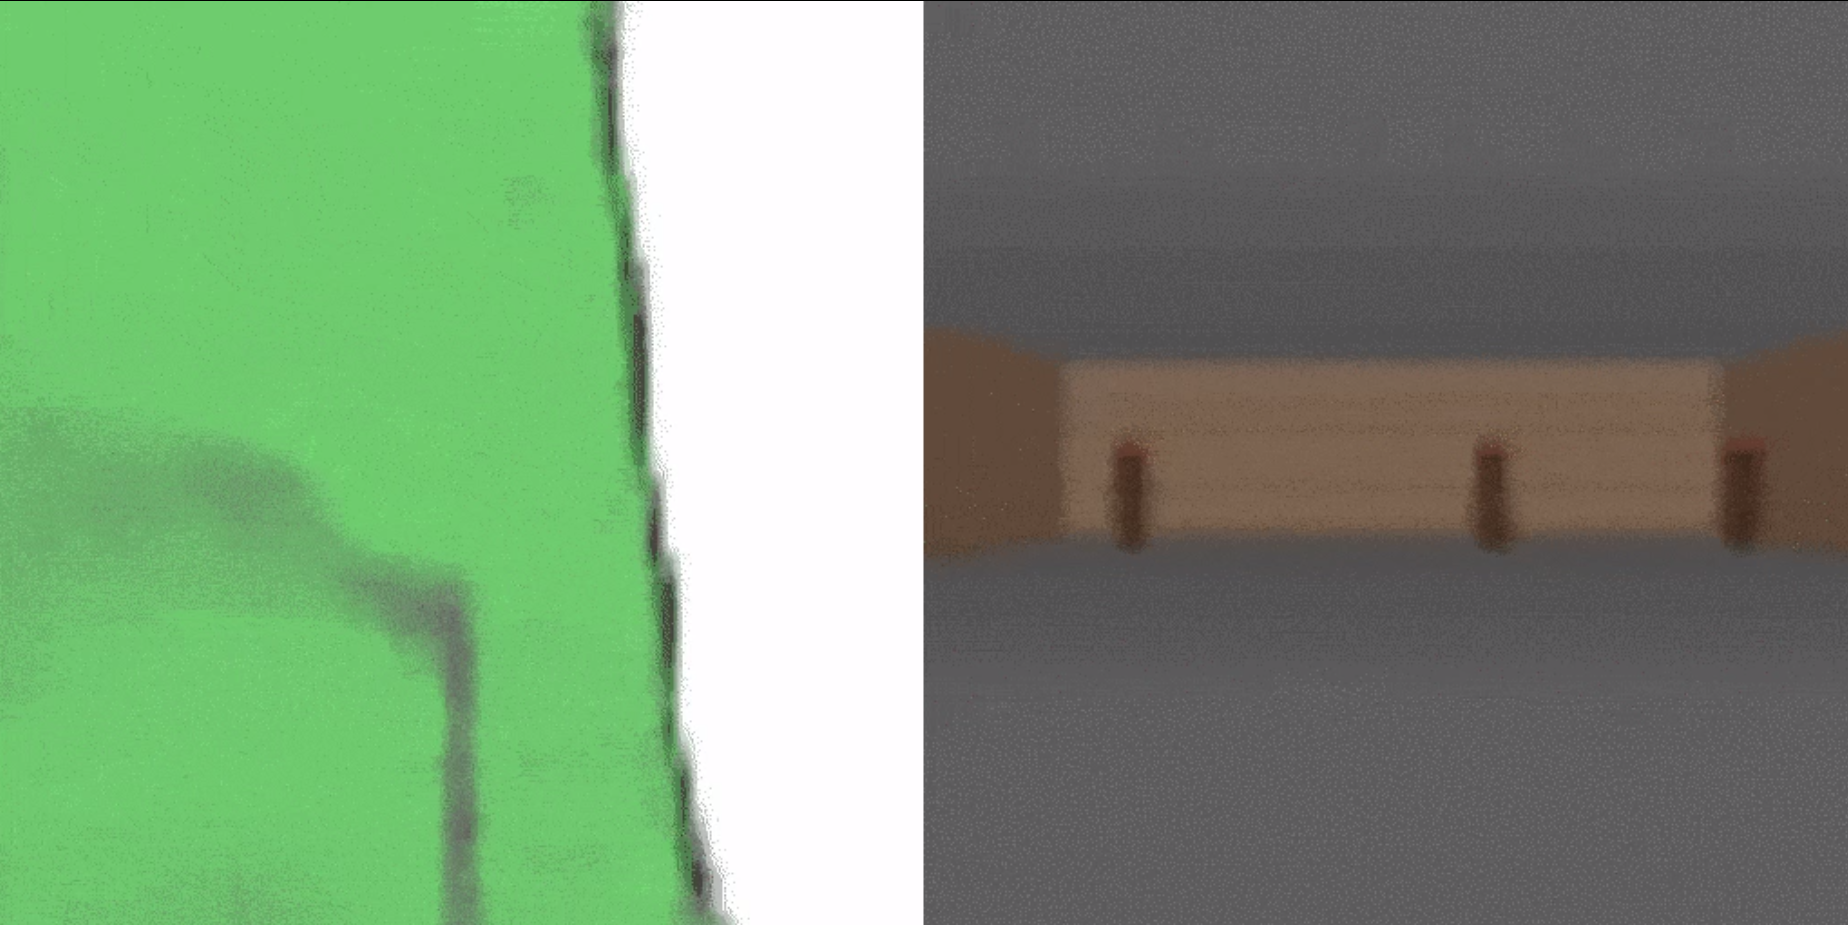
\includegraphics[width=0.8\textwidth]{world_models}}{images/world_models.mp4}
\end{center}

\footnotemark[1]{Ha and Schmidhuber, 2018: ``World Models"}

\end{frame}


\section{2.2.2: Research on Improving Exploration}

\begin{frame}{AKA, the Quest to Solve Montezuma's Revenge}

\begin{center}
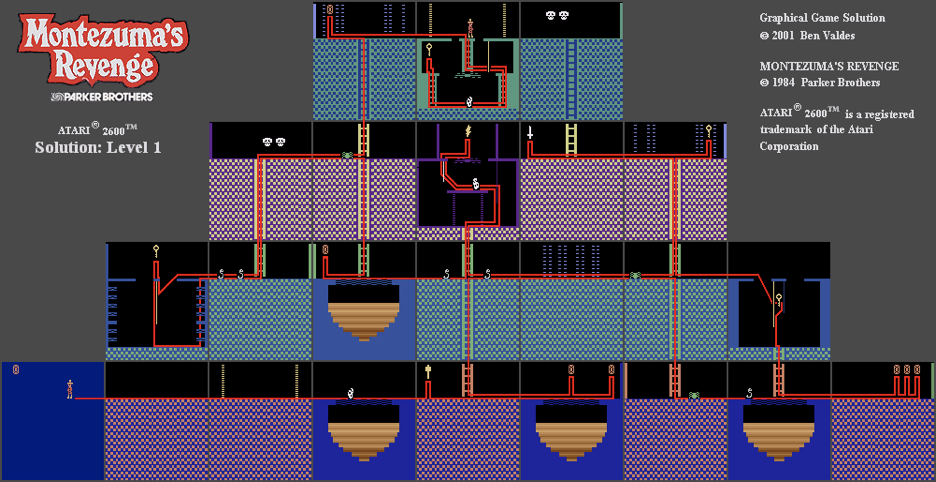
\includegraphics[width=0.9\textwidth]{p2-montezuma}
\end{center}

\begin{itemize}
\item Famously hard Atari game
\item Most RL algorithms do terribly
\item Very sparse rewards, many actions lead to death
\item But humans can do just fine!
\end{itemize}

\end{frame}

\begin{frame}{Intrinsic Motivation}

Various \textbf{intrinsic motivation} schemes exist, which work by adding a non-environment-dependent reward:
%
\begin{equation*}
R(s,a,s') \to R(s,a,s') + \eta R_{int}(s,a,s')
\end{equation*}

Usually, intrinsic reward prefers \textbf{new experiences}. Examples:
%
\begin{itemize}
\item Pseudocount-based methods\footnote{Bellemare et al, 2016: ``Unifying Count-Based Exploration and Intrinsic Motivation"}: approximates number of state visitations with density model, rewards are:
%
\begin{equation*}
R_{int}(s,a,s') \propto \frac{1}{\sqrt{N(s)}}
\end{equation*}
\item Information gain\footnote{Houthooft et al, 2016: ``Variational Information Maximizing Exploration"}: approximates change in info state about environment model based on new experience
%
\begin{equation*}
R_{int}(s,a,s') \approx D_{KL}(P(\calE|\calD_t,s_{t+1})||P(\calE|\calD_t))
\end{equation*}
\end{itemize}

\end{frame}

\begin{frame}{Random Network Distillation}

\textbf{Random Network Distillation}\footnote{Burda et al, 2018: ``Exploration by Random Network Distillation"}: A new and appealingly simple form of intrinsic motivation:
%
\begin{equation*}
R_{int}(s) = \|f_{\phi}(s) - f_{\xi}(s)\|,
\end{equation*}
%
where $f_{\phi}$ is a random neural network (the target) and $f_{\xi}$ is trained to match $f_{\phi}$

\begin{itemize}
\item Exploits generalization properties of networks: $f_{\phi}$ matches $f_{\xi}$ on old states but not new states!
\end{itemize}


\begin{center}
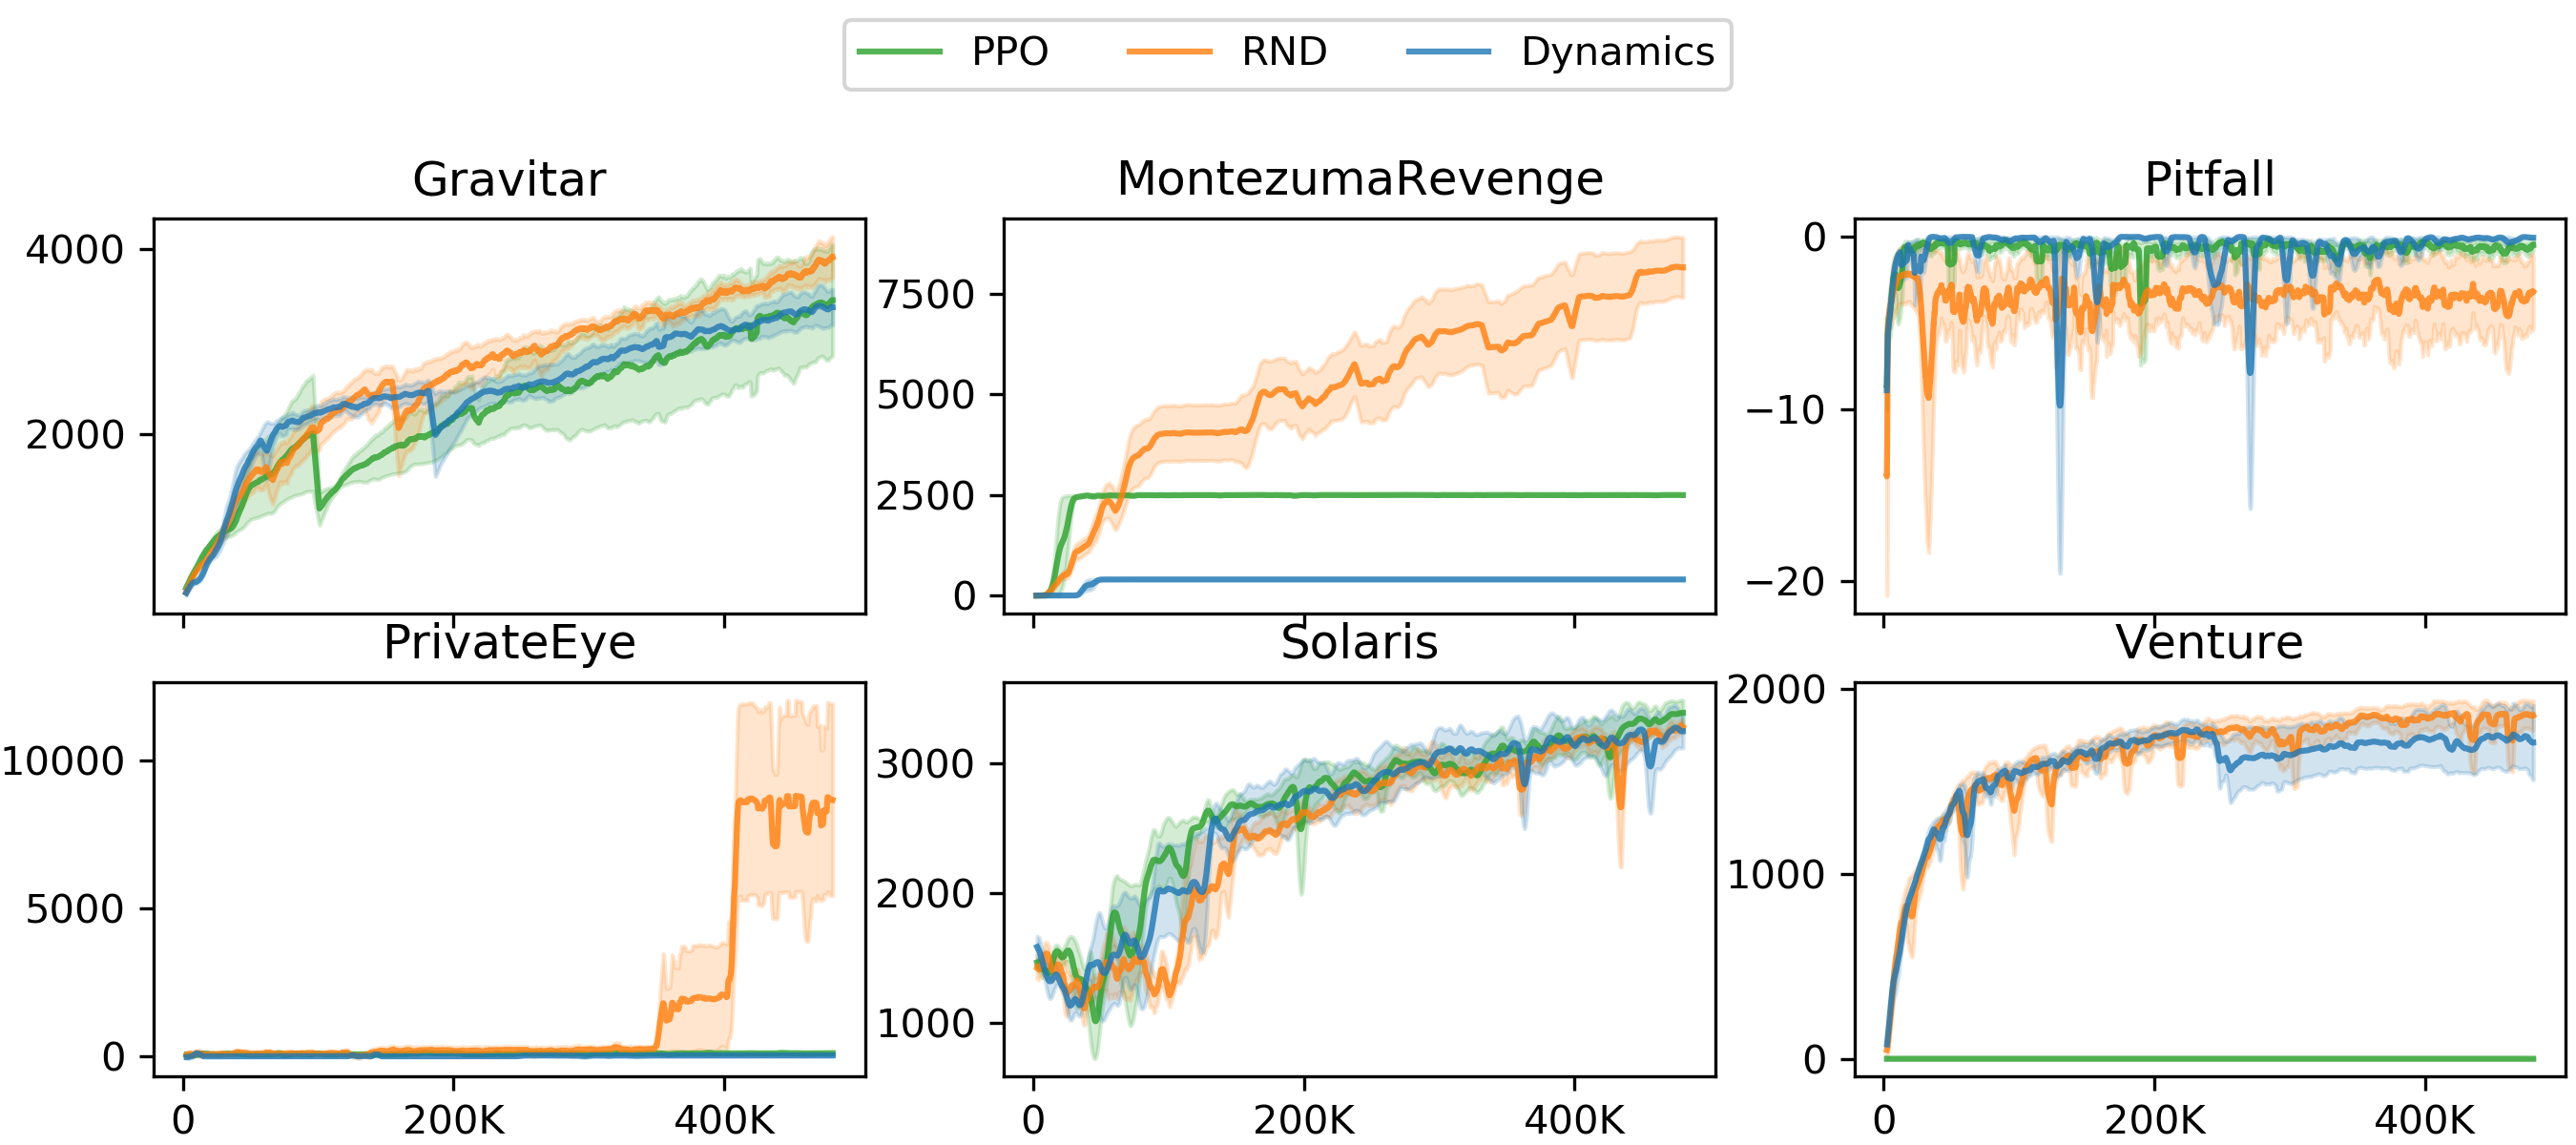
\includegraphics[width=0.8\textwidth]{p2-rnd-atari}
\end{center}
\end{frame}

\begin{frame}{Go-Explore}

Ecoffet et al, 2018 identify a problem with intrinsic motivation that they call \textbf{detachment}:

\begin{center}
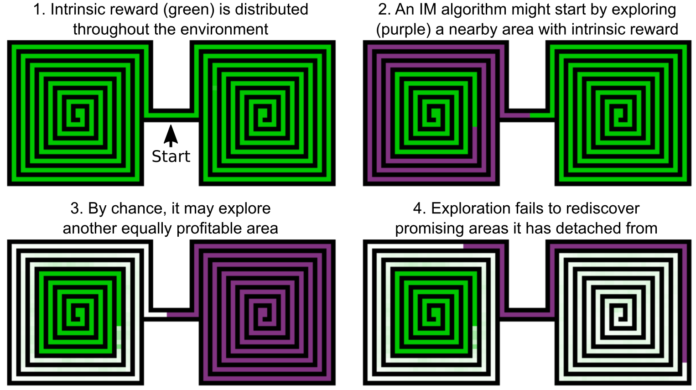
\includegraphics[width=0.8\textwidth]{p2-detach}
\end{center}

\end{frame}

\begin{frame}{Go-Explore}

They rectify detachment with \textbf{Go-Explore}\footnote{Ecoffet et al, 2018: ``Go-Explore: a New Approach for Hard-Exploration Problems"} algorithm:

\begin{center}
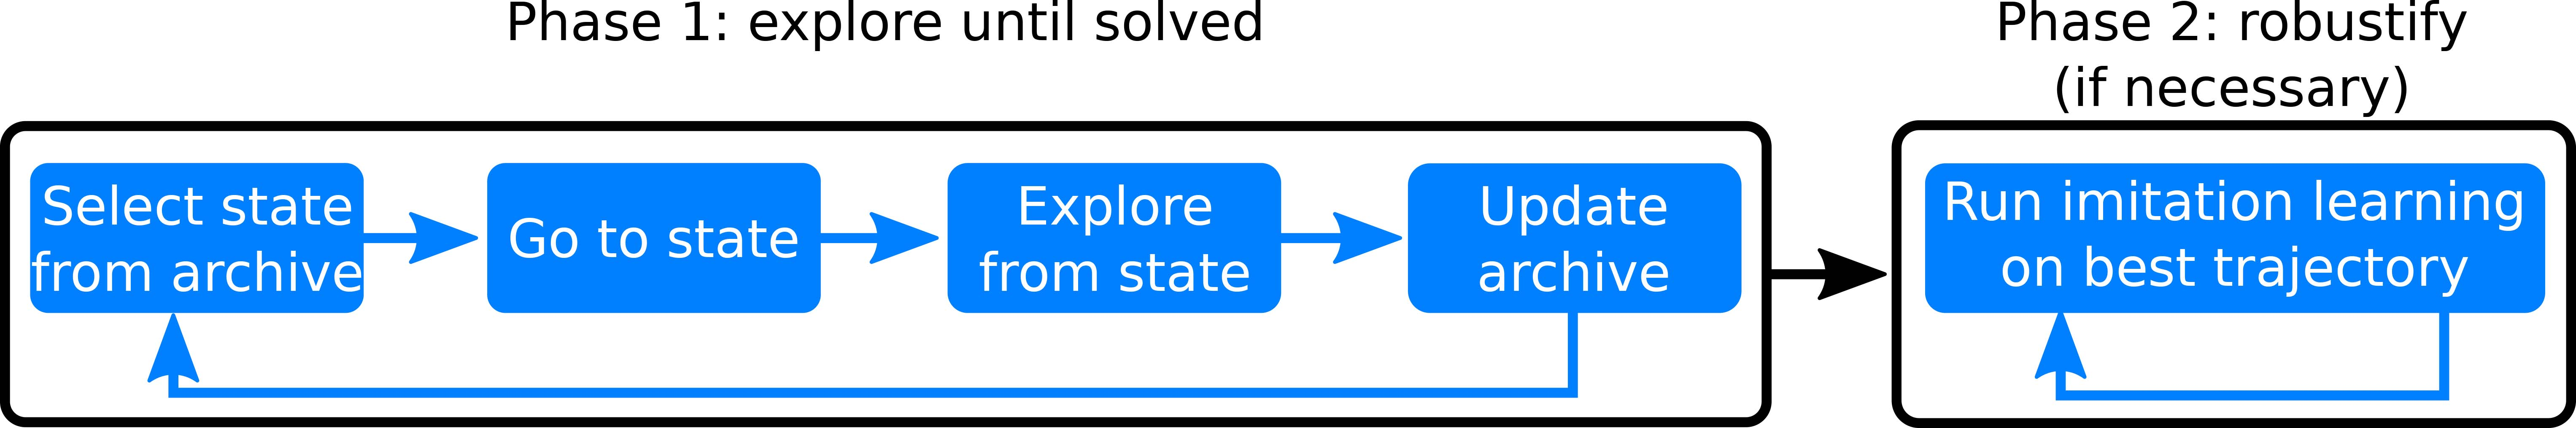
\includegraphics[width=0.8\textwidth]{p2-go-explore}

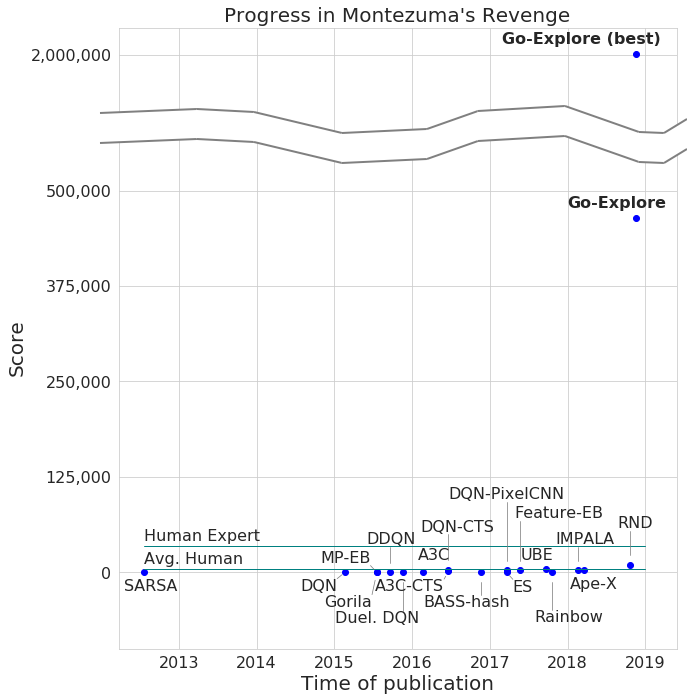
\includegraphics[width=0.4\textwidth]{p2-go-explore2}
\end{center}

\end{frame}


\section{2.3: Spinning Up in Deep RL}

\begin{frame}{Getting started}

If you haven't already:
\begin{itemize}
\item Brush up on math! Be familiar with vectors, matrices, gradients, gradient descent, random variables, expectations, variance, and a few other things.
\item Brush up on deep learning! \textbf{As much as you can get.}
\item Become familiar with TF or PyTorch! \textbf{You need to tinker to learn.}
\item Stay fresh on RL basics! \textbf{Fundamentals go a long way.}
\end{itemize}

\end{frame}
\end{document}